\documentclass[11pt,a4paper]{article}
\usepackage[utf8]{inputenc}
\usepackage[german]{babel}
\usepackage[T1]{fontenc}
\usepackage{amsmath}
\usepackage{amsfonts}
\usepackage{amssymb}
\usepackage{graphicx}
\usepackage[margin=1.25cm]{geometry} % Puts the same margin on all borders of the document

% Packages

\usepackage{hyperref} % Generate hyperlinks to referenced items
\usepackage{adjustbox} % Used to change parameters in \includegraphics[scale=•]{•}
\usepackage{enumitem} % Provides several options for lists
\usepackage{verbatim} % Package to use \begin{comment}
\usepackage{pdfpages} % Used to import PDF pages
\usepackage{multirow} % Allows us to have a single cell in a table span multiple rows
\usepackage{makecell} % Allows us to format multiple lines in a single cell
\usepackage{minted} % Used to syntax highlight code
\usepackage{xcolor}  % Gives access to coloring text
\usepackage{longtable} % Allows us to create a table over multiple pages
\usepackage{float} % Improved placement of floating items
\usepackage{pdfpages} % Used to import pdf pages
\usepackage{booktabs} % Used for horizontal lines instead of \hline



% Settings

\graphicspath{{./files/}} % Sets path for files to the files folder in the same directory

\hypersetup{
    colorlinks=false, %set true if you want colored links
    linktoc=all,     %set to all if you want both sections and subsections linked
    linkcolor=blue,  %choose some color if you want links to stand out
}


\begin{titlepage}
  \title{Rechnerorganisation} % document_name-type_of_document
  \author{Jonas Milkovits}
  \date{Last Edited: \today}
\end{titlepage}

\begin{document}

\pagenumbering{gobble}
\maketitle
\pagenumbering{roman} % i, ii, iii on beginning pages, that don't have content
\tableofcontents
\clearpage
\pagenumbering{arabic} % 1,2,3 on content pages

\section{Einführung}

\subsection{Begrifflichkeiten und Grundlagen}
    \begin{itemize}
        \item \textbf{Abstraktion}
            \begin{itemize}
                \item Wichtiges und zentrales Konzept der Informatik
                \item Verstecken unnötiger Details (für spezielle Aufgabe unnötig)
            \end{itemize}
        
        \item \textbf{Schichtenmodell}
        \item[]
            \begin{minipage}{0.3\textwidth}
            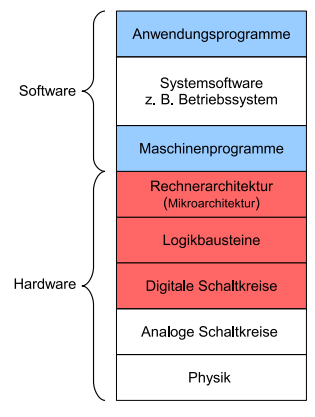
\includegraphics[width=5cm]{schichtenmodell.PNG}
            \end{minipage}
            \begin{minipage}[t]{0.6\textwidth}
            \vspace{-3cm}
                \begin{itemize}
                    \item Untere Schicht erbringt Dienstleistungen für höhere Schicht
                    \item Obere Schicht nutzt Dienste der niedrigeren Schicht
                    \item Eindeutige Schnittstellen zwischen den Schichten
                    \item Vorteile:
                        \begin{itemize}
                            \item Austauschbarkeit einzelner Schichten
                            \item Nur Kenntnis der bearbeitenden Schicht notwendig
                        \end{itemize}
                    \item Nachteile:
                        \begin{itemize}
                            \item ggf. geringere Leistungsfähigkeit des Systems
                        \end{itemize}
                \end{itemize}
            \end{minipage}
        
        \item \textbf{Grundbegriffe}
            \begin{itemize}
                \item Computer:
                    \begin{itemize}
                        \item Datenverarbeitungssystem
                        \item Funktionseinheit zur Verarbeitung und Aufbewahrung von Daten
                        \item Auch Rechner, Informationsverarbeitungssystem, Rechnersystem,..
                        \item Steuerung eines Rechnersystems folgt über ladbares Programm (Maschinenbefehle)
                    \end{itemize}
                \item Grundfunktionen, die ein Rechner ausführt
                    \begin{itemize}
                        \item Verarbeitung von Daten (Rechnen, logische Verknüpfungen,..)
                        \item Speichern von Daten (Ablegen, Wiederauffinden, Löschen)
                        \item Umformen von Daten (Sortieren, Packen, Entpacken)
                        \item Kommunizieren (Mit Benutzer, mit anderen Rechnersystemen)
                    \end{itemize}
            \end{itemize}

        \item \textbf{Komponenten eines Rechnersystems}
            \begin{itemize}
                \item Prozessor
                    \begin{itemize}
                        \item Zentraleinheit, Central Processing Unit (CPU)
                        \item Ausführung von Programmen
                    \end{itemize}
                \item Speicher
                    \begin{itemize}
                        \item Enthält Programme und Daten (Speichersystem)
                    \end{itemize}
                \item Kommunikation
                    \begin{itemize}
                        \item Transfer von Informationen zwischen Speicher und Prozessor
                        \item Kommunikation mit der Außenwelt (Ein-/Ausgabesystem)
                    \end{itemize}
                \item[] 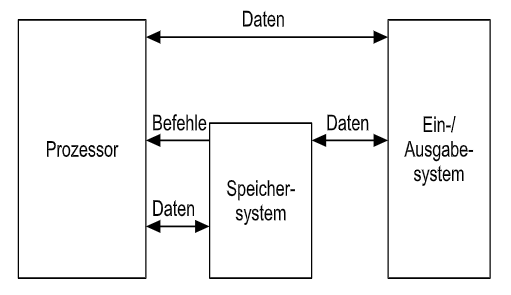
\includegraphics[width=8cm]{rechnersystem.PNG}
            \end{itemize}

        \item \textbf{Nähere Informationen zum Speicher} 
            \begin{itemize}
                \item Explizite Nutzung des Speichersystem
                    \begin{itemize}
                        \item Interne Prozessorspeicher/Register
                            \begin{itemize}
                                \item schnelle Register zur temporären Speicherung von Daten/Befehlen
                                \item direkter Zugriff durch Maschinenbefehle
                                \item Technologie: Halbleiter ICs
                            \end{itemize}
                        
                        \item Hauptspeicher
                            \begin{itemize}
                                \item relativ großer und schneller Speicher für Programme/Daten 
                                \item direkter Zugriff durch Maschinenbefehle 
                                \item Technologie: Halbleiter ICs
                            \end{itemize}

                        \item Sekundärspeicher
                            \begin{itemize}
                                \item großer, aber langsamer Speicher für permanente Speicherung
                                \item indirekter Zugriff über E/A-Programme (Daten $\rightarrow$ Hauptspeicher)
                                \item Technologie: Halbleiter ICs, Magnetplatten, optische Laufwerke
                                \item z.B.: Festplatte
                            \end{itemize}
                    \end{itemize}

                \item Implizite (transparente) Nutzung 
                    \begin{itemize}
                        \item Für das Maschinenprogramm transparent
                        \item bestimmte Register auf dem Prozessor 
                        \item Cache-Speicher
                    \end{itemize}
                
                \item[] 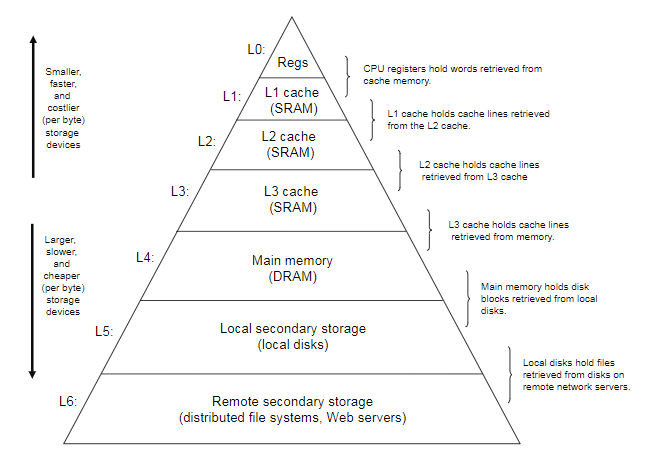
\includegraphics[width=12cm]{speicherhierarchie}
                
                \item Speicherorganisation: Big-Endian und Little-Endian 
                \item[]
                    \begin{minipage}{0.2\textwidth}
                    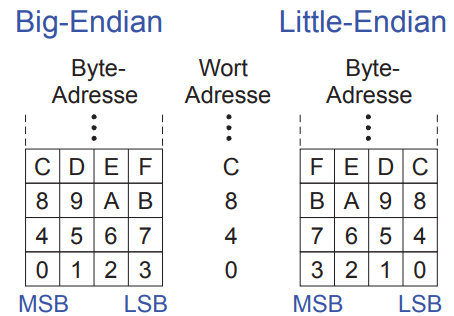
\includegraphics[width=4cm]{bigLittleEndian.PNG}
                    \end{minipage}
                    \begin{minipage}[t]{0.7\textwidth}
                    \vspace{-1.2cm}
                        \begin{itemize}
                            \item Schemata für Nummerierung von Bytes in einem Wort
                            \item Big-Endian: Bytes werden vom höchstwertigen Ende gezählt
                            \item Little-Endian: Bytes werden vom niederstwertigen Ende gezählt
                        \end{itemize}
                    \end{minipage}
            \end{itemize}
            
    \end{itemize}

\pagebreak

\subsection{Streifzug durch die Geschichte}

    \begin{itemize}
        \item \textbf{Übersicht über die geschichtliche Entwicklung mit wichtigsten Meilensteinen}
        \begin{itemize}
            \item[] 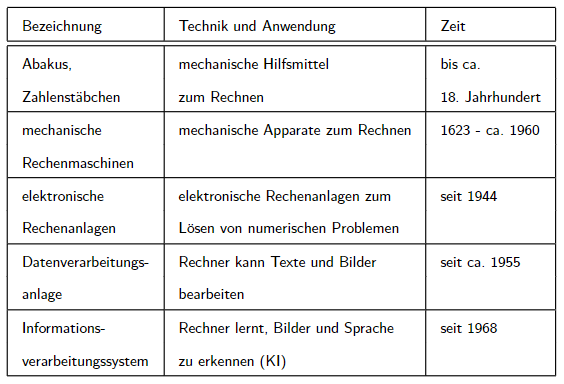
\includegraphics[width=12cm]{geschichtsTabelle1.PNG}
        \end{itemize}
        
        \item \textbf{Fünf Rechnergenerationen im Überblick:}
            \begin{itemize}
                \item[] 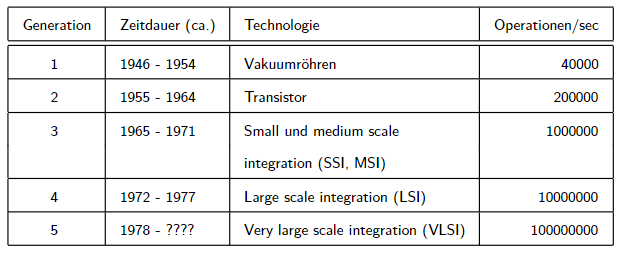
\includegraphics[width=12cm]{rechnergenerationen} 
            \end{itemize}
        
        \item \textbf{Rechner im elektronischen Zeitalter}
            \begin{itemize}
                \item 1954: Entwicklung der Programmiersprache Fortran
                \item 1955: Erster Transistorrechner
                \item 1957: Entwicklung Magnetplattenspeicher, Erste Betriebssysteme für Großrechner
                \item 1968: Erster Taschenrechner
                \item 1971: Erster Mikroprozessor
                \item 1981: Erster IBM PC, Beginn des PC-Zeitalters
            \end{itemize}
    \end{itemize}

\subsection{Ethik in der Informatik}

    \begin{itemize}
        \item Ethik in der Informatik
            \begin{itemize}
                \item Ethik: Bewertung menschlichen Handelns
                \item Verbindung zur Informatik: Anwendung von Rechnern für kriegisches Handelns
                \item \textbf{Dual-Use-Problematik}: Verwendbarkeit von Rechnern für zivile als auch militärische Zwecke
            \end{itemize}
        
        \item Digitale Souveränität
            \begin{itemize}
                \item Souveränität: Fähigkeit zur Selbstbestimmung (Eigenständigkeit, Unabhängigkeit)
                \item Digitale Souveränität: Souveränität im digitalen Raum
            \end{itemize}
    \end{itemize}

\section{Einführung in die maschinennahe Programmierung}
\subsection{Begrifflichkeiten und Grundlagen}
    \begin{itemize}
        \item \textbf{Allgemein}
            \begin{itemize}
                \item Architektur / Programmiermodell
                    \begin{itemize}
                        \item Programmierersicht auf Rechnersystem 
                        \item Definiert durch Maschinenbefehle und Operanden
                    \end{itemize}
                \item Mikroarchitektur
                    \begin{itemize}
                        \item Hardware-Implementierung der Architektur
                    \end{itemize}
            \end{itemize}
        
        \item \textbf{Programmierparadigmen}
            \begin{itemize}
                \item Synonyme: Denkmuster, Musterbeispiel
                \item Bezeichnet in der Informatik ein übergeordnetes Prinzip
                \item Dieses Prinzip ist für eine ganze Teildisziplin typisch
                \item Manifestiert sich an Beispielen, keine konkrete Formulierung
                \item Maschinensprache (Assembler) ist ein primitives Paradigma              
            \end{itemize}

        \item \textbf{Programmiermodell}
            \begin{itemize}
                \item Bei höheren Programmiersprachen:
                    \begin{itemize}
                        \item Grundlegende Eigenschaften einer Programmiersprache 
                    \end{itemize} 
                \item Bei maschinennaher Programmierung:
                    \begin{itemize}
                        \item Bezeichnet dort den \textbf{Registersatz} eines Prozessors 
                        \item Registersatz besteht aus:
                            \begin{itemize}
                                \item Register, die durch Programme angesprochen werden können
                                \item Liste aller verfügbaren Befehle (\textbf{Befehlssatz})
                            \end{itemize}
                        \item Register, die prozessorintern verwendet werden (IP/PC) zählen nicht zum Registersatz
                            \begin{itemize}
                                \item IC: Instruction Pointer 
                                \item PC: Program Counter
                            \end{itemize}
                    \end{itemize}
            \end{itemize}

        \item \textbf{Verfeinerung des Rechensystems}
            \begin{itemize}
                \item[] 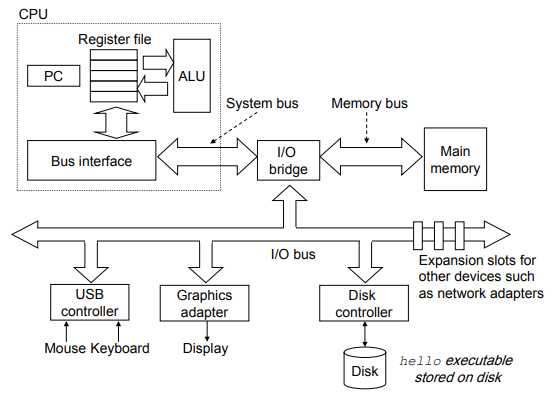
\includegraphics[width=9cm]{modernesRechnersystem.PNG}
                \item {\makebox[6cm][l]{CPU/Prozessor:}} führt die im Hauptspeicher abgelegten Befehle aus 
                \item {\makebox[6cm][l]{ALU/Arithmethic Logical Unit:}} Ausführung der Operationen
                \item {\makebox[6cm][l]{PC/Program Counter:}} Verweis auf nächsten Maschinenbefehl im Hauptspeicher
                \item {\makebox[6cm][l]{Register:}} Schneller Speicher für Operanden
                \item {\makebox[6cm][l]{Hauptspeicher:}} Speichert Befehle und Daten 
                \item {\makebox[6cm][l]{Bus Interface:}} Verbinden der einzelnen Komponenten
            \end{itemize}

        \item \textbf{Assembler}
            \begin{itemize}
                \item Programmieren in der Sprache des Computers
                    \begin{itemize}
                        \item {\makebox[3cm][l]{Maschinenbefehle:}} Einzelnes Wort
                        \item {\makebox[3cm][l]{Befehlssatz:}} Gesamtes Vokabular
                    \end{itemize}
                \item Befehle geben Art der Operation und ihre Operanden an 
                \item Zwei Darstellungen:
                    \begin{itemize}
                        \item Assemblersprache: Für Menschen lesbare Schreibweise für Instruktionen
                        \item Maschinensprache: maschinenlesbares Format (1 und 0)
                    \end{itemize}
            \end{itemize}
        
        \item \textbf{ARM-Architektur - Hier verwendetes Rechnersystem}
            \begin{itemize}
                \item z.B. verwendet bei Raspberry Pi 
                \item ARM: Acorn RISC Machines / Advanced RISC Machines 
                \item Große Verbreitung heutzutage in Smartphones
            \end{itemize}

    \end{itemize}



\subsection{Phasen der Übersetzung}

        \begin{itemize}
            \item Beispielhaftes \texttt{C}-Programm:
            \item[]
                \begin{minted}[autogobble]{c}
                #include<stdio.h> /* Standard Input/Output */ /* Header-Datei*/
                int main() {
                printf("Hello World\n");
                return 0;
                }
                \end{minted}
            \item \texttt{C}-Programm an sich für den Menschen verständlich
            \item Übersetzung in Maschinenbefehle für Ausführung auf dem Rechnersystem:
            \item[] \includegraphics[width=12cm]{übersetzungsPhasen.PNG}
            \item 1. Phase \textbf{(Preprocessor)}
                \begin{itemize}
                    \item Aufbereitung durch Ausführung von Direktiven (Code mit \#)
                    \item z.B.: Bearbeiten von \texttt{\#include <stdio.h>}
                        \begin{itemize}
                            \item Lesen des Inhalts der Datei \texttt{stdio.h}
                            \item Kopieren des Inhalts in die Programmdatei
                        \end{itemize}
                    \item Ausgabe: \texttt{C}-Programm mit der Endung \texttt{.i} 
                \end{itemize}
            
            \item 2. Phase \textbf{(Compiler)}
                \begin{itemize}
                    \item Übersetzt \texttt{C-}Programm \texttt{hello.i} in Assemblerprogramm \texttt{hello.s}
                \end{itemize}
            \item 3. Phase \textbf{(Assembler)}
                \begin{itemize}
                    \item Übersetzt \texttt{hello.s} in Maschinensprache
                    \item Ergebnis ist das Objekt-Programm \texttt{hello.o}
                \end{itemize}
            \item 4. Phase \textbf{(Linker)}
                \begin{itemize}
                    \item Zusammenfügen verschiedener Module
                        \begin{itemize}
                            \item Code von \texttt{printf} exisitert bereits als \texttt{print.o}-Datei
                        \end{itemize}
                    \item Linker kombiniert \texttt{hello.o} und \texttt{printf.o} zu ausführbarem Programm
                    \item Ausgabe des Bindevorgangs: ausführbare \texttt{hello}-Objektdatei
                \end{itemize}
        
        \end{itemize}



\subsection{Ausführung eines Programms im Rechnersystem}
        
        \begin{itemize}
            \item Ausgangspunkt
                \begin{itemize}
                    \item Ausführbares Objektprogramm \texttt{hello} auf der Festplatte 
                    \item Starten der Ausführung des Programms unter Nutzung der Shell 
                \end{itemize}
            
            \item Ablauf:
                \begin{itemize}
                    \item Shell liegt Zeichen des Kommandos ins Register
                    \item Speichert den Inhalt dann im Hauptspeicher ab
                    \item[] \includegraphics[width=9cm]{ausführung1.PNG}
                    \item Schrittweises Kopieren der Befehle/Daten von Festplatte in Hauptspeicher
                    \item[] \includegraphics[width=9cm]{ausführung2.PNG}
                    \item Ausführen der Maschinenbefehle des \texttt{hello}-Programms
                    \item[] \includegraphics[width=9cm]{ausführung3.PNG} 
                \end{itemize}
        \end{itemize}


\pagebreak

\subsection{Befehle eines Rechnersystems}
    \begin{itemize}
        \item Wieviele Befehle und was für Befehle soll ein Rechnersystem haben?
        \item Viele komplexe Befehle: 
            \begin{itemize}
                \item \textbf{CISC-Maschinen} (Complex Instruction Set Computer)
                \item Befehlsausführung direkt im Speicher möglich
                \item Verwendet von Intel-Architektur 
            \end{itemize}
        \item Weitgehend identische Ausführungszeit der Befehle
            \begin{itemize}
                \item \textbf{RISC-Maschinen} (Reduce Instruction Set Computer)
                \item Ermöglicht effizientes Pipeling
                \item Werden auch als Load/Store-Architekturen bezeichnet (Nur Ausführung im Register)
                \item Verwendet von ARM-Architektur
            \end{itemize}
        \item Jedoch viele Befehle, die jeder Prozessor hat (AND, OR, NOT,..)
        \item Unterschiedliche Befehlsformate:
            \begin{itemize}
                \item Erlauben Flexibilität
                \item z.B. \texttt{add} und \texttt{sub} mit drei Registern als Operanden
                \item z.B. \texttt{ldr} und \texttt{str} verwenden zwei Register und Konstante
                \item Anzahl an Formaten sollte jedoch klein sein 
                    \begin{itemize}
                        \item Hardware weniger aufwendig
                        \item Erlaubt evtl. höhere Verarbeitungsgeschwindigkeit
                    \end{itemize}
            \end{itemize}
        \item Interner Aufbau eines Rechners hat viele Freiheitsgrade
        \item Diese Struktur hat erheblichen Einfluss auf die Leistungsfähigkeit eines Rechnersystems 
        \item \textbf{$n$-Adressmaschinen}
            \begin{itemize}
                \item Einteilung nach der Anzahl der Operanden in einem Maschinenbefehl 
                \item 2-Adressmaschine (Intel Architektur)
                \item 3-Adressmaschine (ARM Architektur)
            \end{itemize}
        \item \textbf{Konstanten in Befehlen (immediates)}
            \begin{itemize}
                \item Direkt im Befehl untergebebracht $\rightarrow$ Direktwerte
                \item Benötigen kein eigenes Register oder Speicherzugriff
                \item Direktwert ist Zweierkomplementzahl, die 12 Bit breit ist 
                \item Bitbreite der Direktwertzahl vom Befehl abhängig
                    \begin{itemize}
                        \item Befehle haben immer 32 Bit
                        \item Registeradressen werden mit 4 Bit kodiert
                        \item Übrigbleibende Bits für Direktwert
                    \end{itemize}
            \end{itemize}
    \end{itemize}

\subsection{Registersatz}
    \begin{itemize}
        \item[]
            \begin{minipage}{0.2\textwidth}
            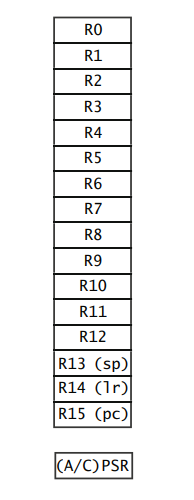
\includegraphics[width=3cm]{registersatz.PNG}
            \end{minipage}
            \begin{minipage}[t]{0.7\textwidth}
            \vspace{-3cm}
                \begin{itemize}
                    \item R0: Verwendet für Rückgabe von Werten an die \texttt{Shell}
                    \item R1-R12: General Purpose Register
                    \item R13: Stack Pointer (sp)
                    \item R14: Link Register (lr)
                    \item R15: Program Counter (pc)
                    \item Current Processor Status Register (CPSR)
                \end{itemize}
            \end{minipage}
        \item \textbf{Current Processor Status Register}
            \begin{itemize}
                \item Enthält unter anderem die \texttt{Statusflags}
                \item[] 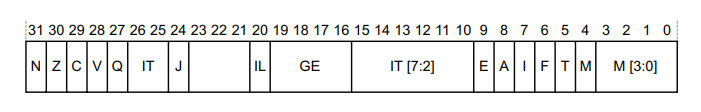
\includegraphics[width=15cm]{statusflags}
                \item Werden oft für Vergleiche (\texttt{b,beq,...}) verwendet 
                \item \texttt{N} (Negative): Wird verwendet um zu zeigen, dass Ergebnis negativ ist
                \item \texttt{Z} (Zero): Wird verwendet um zu zeigen, dass Ergebnis 0 ist 
                \item \texttt{C} (Carry): Zeigt, dass Carry-Bit besteht 
                \item \texttt{V} (OverFlow): Zeigt, dass Overflow geschehen ist 
                \item Namen können je nach Prozessor stark variieren
            \end{itemize}
    \end{itemize}



\subsection{Adressierung des Speichers, Lesen und Schreiben auf Speicher}
    \begin{itemize}
        \item \textbf{Allgemeine Verwendung von Registerspeicher}
            \begin{itemize}
                \item Meist zuviele Daten für die Register 
                \item Kombination des Registers und Hauptspeichers zum Halten von Daten 
                \item Speichern von häufig verwendeten Daten in Registern (Schleifenvariable)
            \end{itemize}
        
\pagebreak

        \item \textbf{Wort- und Byte-Adressierung von Daten im Speicher }
            \begin{itemize}
                \item Byte-adressiert: (ARM)
                    \begin{itemize}
                        \item Jedes Byte hat eine eindeutige Adresse (Zugriff auf jedes Byte möglich)
                        \item Ein Wort (hier 32Bit) besteht aus 4 Bytes (32 Bits)
                        \item Wortbreite ist von der Architektur abhängig
                        \item Wortadressen sind immer Vielfache von 4 (Offset von 4)
                        \item[]
                        \item[] 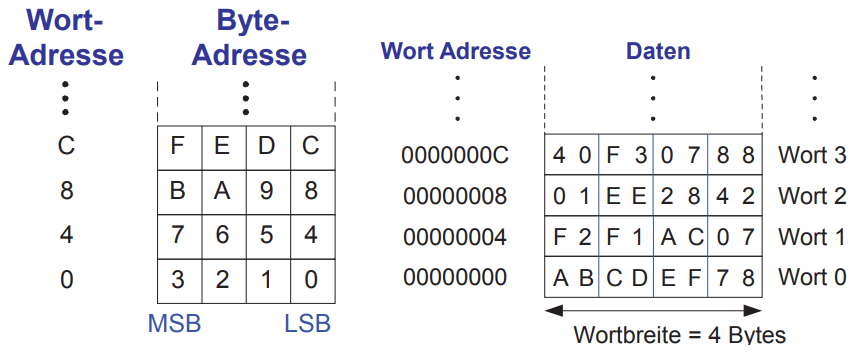
\includegraphics[width=12cm]{wortAdresse.PNG}
                        \item Rechts wird ein Byte mit zwei Hexawerten dargestellt ($AB:~1011~1010$)
                    \end{itemize}
            \end{itemize}
        
        \item \textbf{Lesen aus byte-adressiertem Speicher}
            \begin{itemize}
                \item Lesen geschieht durch Ladebefehle (Transportbefehl)
                \item Befehlsname: \texttt{load word (ldr)}
                \item Alternative für Bytes statt Wörtern: \texttt{ldrb}
                \item Adressarithmethik: 
                \begin{itemize}
                    \item Adressen werden relativ zu Register angegeben
                    \item Basisadresse (startet bei Wort 0) plus Distanz (offset)
                    \item Adresse = \texttt{(r5 (Basis) + 8 (offset))}
                \end{itemize}
                \item Beispiel 1:
                    \begin{itemize}
                        \item Lese Datenwort von Speicheradresse \texttt{(r5+8)} und schreibe es in Register \texttt{r7}
                        \item[]
                            \begin{minted}[autogobble]{c}
                            mov r5,#0 /* Transportbefehl, schreibt Konstante 0 in r5 */
                            ldr r7, [r5,#8] /* r7: Zielregister | [r5,#8] Quelle */
                            \end{minted}
                        \item \texttt{r7} enthält das Datenwort der Speicheradresse \texttt{r5+8}
                    \end{itemize}
                \item Beispiel 2:
                    \begin{itemize}
                        \item Lesen Datenwort 3 (Speicheradresse \texttt{0xC} (12er Offset)) nach \texttt{r7}
                        \item (Einschub: \texttt{0x} sagt dem Compiler, dass das Folgende eine Hexzahl ist)
                        \item[]
                            \begin{minted}[autogobble]{c}
                            mov r5,#0 /* Schreibt Konstante 0 in r5 */
                            ldr r7, [r5, #0xC] /* Lädt den Wert (r5+12) in r7 */
                            \end{minted}
                        \item Nach Abarbeiten des Befehls hat \texttt{r7} den Wert \texttt{0x40F30788}
                        \item[]
                        \item[] 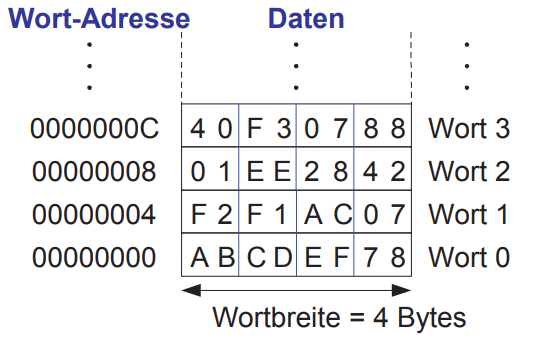
\includegraphics[width=8cm]{byteAdresseBsp2}
                    \end{itemize}
            \end{itemize}

        \item \textbf{Schreiben in byte-adressierten Speicher}
            \begin{itemize}
                \item Schreiben geschieht durch Speicherbefehle (Transportbefehl)
                \item Befehlsname: \texttt{store word (str)}
                \item Alternative für Bytes statt Wörtern: \texttt{strb}
                \item Beispiel:
                    \begin{itemize}
                        \item Schreibe den Wert aus \texttt{r9} in Speicherwort 5
                        \item[]
                            \begin{minted}[autogobble]{c}
                            mov r1,#0 /* Speichert Konstante 0 in r1 */
                            mov r9,#42 /* Speichert Konstante 42 in r9 */
                            str r9, [r1,#0x14] /* Schreibt Wert des 5. Wortes von r1 in r9 */
                            \end{minted}
                        \item \texttt{\#0x14}: $14_{16} = 0001~0100_2 = 20_{10}$ (5.tes Wort)
                    \end{itemize}
            \end{itemize}
    \end{itemize}
        
\subsection{Kontrollstrukturen in Assembler}
    \begin{itemize}
        \item \textbf{Statusbits}
            \begin{itemize}
                \item Die Wichtigsten:
                    \begin{itemize}
                        \item \texttt{CF (CarryFlag)}
                        \item \texttt{ZF (ZeroFlag)}
                        \item \texttt{SF (SignFlag)}
                        \item \texttt{OF (OverflowFlag)}
                    \end{itemize}
                \item Verwendung:
                    \begin{itemize}
                        \item Vergleiche (\texttt{cmp})
                        \item Gleichheit
                    \end{itemize}
                \item Unterschiede zwischen \texttt{Carry} und \texttt{Overflow}
                    \begin{itemize}
                        \item \texttt{Overflow}: Ergebnis passt nicht in maximale darstellbare Werte (z.B. +8 bei 4 Bit im ZK)
                        \item \texttt{Carry}: Ergebnis passt nicht in Bitbreite ( +5 - 1 = +4)
                        \item \texttt{Sign}: Vorzeichen negativ
                    \end{itemize}
            \end{itemize}
        
        \item \textbf{Sprünge / Verzweigungen}
            \begin{itemize}
                \item Änderung der Ausführungsreihenfolge von Befehlen 
                \item Unbedingte Sprünge
                    \begin{itemize}
                        \item Werden immer ausgeführt
                        \item \mint{c}|b target /* Springt von branch zu target */| 
                    \end{itemize}
                \item Bedingte Sprünge
                    \begin{itemize}
                        \item Sprünge abhängig von Bedingung 
                        \item \mint{c}|beq target /* Ein Beispiel, eq für equal */| 
                    \end{itemize}
                \item Label 
                    \begin{itemize}
                        \item Label sind Namen für Adressen im Programm 
                        \item Name muss unterschiedlich von Maschinenbefehlen (Mnemonics) sein 
                        \item Label müssen mit einem Doppelpunkt abgeschlossen werden
                        \item Werden zur Markierung von Stellen für Sprünge verwendet (target)
                    \end{itemize}
            \end{itemize}
        
        \item \textbf{Bedingte Sprünge}
            \begin{itemize}
                \item[]
                    \begin{minted}[autogobble]{c}
                    mov r0,#4       /* r0 = 4 */
                    add r1,r0,r0    /* r1 = 8 */ 
                    cmp r0, r1      /* r0 - r1 = -4: NZCV = 1000 */
                                    /* StatusBits NZCV */
                    beq there       /* Kein Sprung: Z != 1 */
                                    /* Müsste bei Gleichheit (equal) 0 sein */
                    add r1,r1,#42   /* r1 = r1 + 42 */

                    there:
                    add r1,r1,#78   /* r1 = r1 + 78 */
                    \end{minted}
                \item Weitere Bedingungen: 
                    \begin{itemize}
                        \item \texttt{beq}: Equal / Gleichheit 
                        \item \texttt{bne}: Not Equal / Ungleichheit
                        \item \texttt{bge}: Greater / Größer
                        \item \texttt{ble}: Less / Kleiner
                    \end{itemize}
            \end{itemize}
        
        \item \textbf{if-Anweisung}
            \begin{itemize}
                \item[]
                    \begin{minted}[autogobble]{c}
                    /* r0 = 5; r1 = 10; r2 = f; r3 = i */
                    cmp r0,r1       /* Vergleicht r0 und r1 */ 
                    bne L1          /* Falls Werte ungleich sind, ist hier gegeben */
                    add r2,r3,#1    /* Wird hier übersprungen */
                    L1:             /* Hierhin wird gesprungen */
                    sub r2,r2,r3 
                    \end{minted}
            \end{itemize}

        \item \textbf{if/else-Anweisung}
            \begin{itemize}
                \item[]
                    \begin{minted}[autogobble]{c}
                    /* r0 = 5; r1 = 10; r2 = f; r3 = i */
                    cmp r0,r1 
                    bne L1          /* Potentieller Sprung nach L1 */
                    add r2,r3,#1    /* else-Anweisung (wird übersprungen, falls Bedingung korrekt) */
                    b L2            /* Überspringen der if-Anweisung, sonst wird beides ausgeführt */
                    L1:
                    sub r2,r2,r3 
                    L2:
                    ...
                    \end{minted}
            \end{itemize}

        \item \textbf{while-Schleifen}
            \begin{itemize}
                \item[]
                    \begin{minted}[autogobble]{c}
                    /* r0 = pow; r1 = x */
                    mov r0,#1
                    mov r1,#0
                    WHILE:          /* Label für Schleife*/
                    cmp r0,#128     /* Abbruchbedingung: Falls equal Z = 1 */
                    beq DONE        /* Sprung aus Schleife */   
                    lsl r0,r0,#1    /* Linksshift um 1 Bit / Schleifencode */
                    add r1,r1,#1    /* x = x + 1 / Schleifencode */
                    b WHILE         /* Fortführen der Schleife */
                    DONE:
                    ...
                    \end{minted}
            \end{itemize}

        \item \textbf{for-Schleifen}
            \begin{itemize}
                \item[]
                    \begin{minted}[autogobble]{c}
                    /* r0 = i; r1 = sum */
                    mov r1,#0
                    mov r0,#0
                    FOR:            /* Label für Schleife */
                    cmp r0,#10      /* Abbruchbedingung: Falls i größer als 10 ist */
                    bge DONE 
                    add r1,r1,r0    /* sum = sum + i */
                    add r0,r0,#1    /* i = i + 1 */
                    b FOR           /* Fortführen der Schleife */
                    DONE:
                    ...
                    \end{minted}
            \end{itemize}
    \end{itemize}

\pagebreak

\subsection{Nutzung des Hauptspeichers}
    \begin{itemize}
        \item \textbf{Erklärung anhand eines Codebeispiels}
            \begin{itemize}
                \item[] 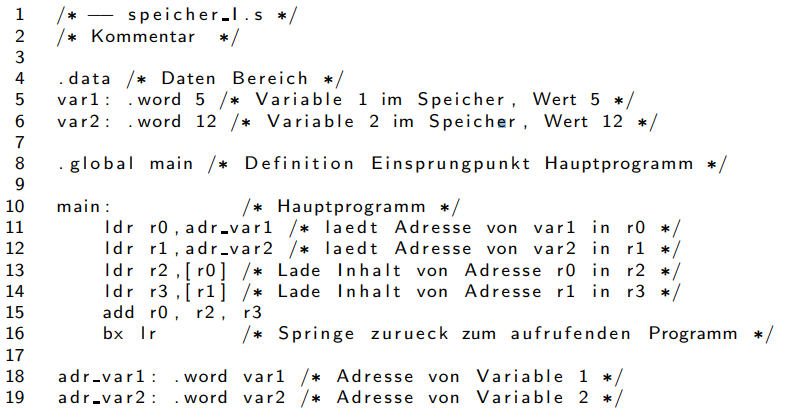
\includegraphics[width=15cm]{codeBeispielHauptspeicher1}
                \item \texttt{.data (Zeile 4)}: 
                    \begin{itemize}
                        \item Variablen, die im Speicher (nicht im Register) abgelegt werden
                        \item \texttt{.word}: Festlegung des Typs (hier 32 Bit)
                        \item Name \texttt{var1}: An sicht frei wählbar
                    \end{itemize}

                \item \texttt{.global main (Zeile 8)}:
                    \begin{itemize}
                        \item Definiert das Label, das als Einsprungspunkt gilt (hier \texttt{main})
                    \end{itemize}

                \item \texttt{adr\_var1: .word var1 (Zeile 18/19)}:
                    \begin{itemize}
                        \item Hier werden die Adressen der Variablen im Speicher in einer Variable abgespeichert
                        \item Wichtig: Unterscheidung zwischen Adresse und Wert
                    \end{itemize}

                \item \texttt{ldr r0, adr\_var1 (Zeile 11)}:
                    \begin{itemize}
                        \item Lädt nun die Adresse unseres Hauptspeicherwertes in ein Register
                        \item Hierfür nutzen wir die eben erstellte \texttt{adr\_var1}
                    \end{itemize}

                \item \texttt{ldr r2,[r0] (Zeile 13)}:
                    \begin{itemize}
                        \item Lädt den Inhalt der Adresse in \texttt{r0} in \texttt{r2}
                        \item Verwendung von \texttt{[]} um dies anzuzeigen
                    \end{itemize}

                \item Variationen:
                    \begin{itemize}
                        \item Zeile 13: \texttt{ldr r2,[r0,\#4]}
                            \begin{itemize}
                                \item Hinzufügen eines Offsets beim Laden des Wertes 
                                \item Dies führt dazu, dass der Wert auf \texttt{r1} geladen wird (12)
                                \item Ausgabe des Programms ist damit 24, statt 17
                            \end{itemize}
                        \item \texttt{mov r5,\#4} | \texttt{ldr r2,[r0,r5]}
                            \begin{itemize}
                                \item In Registern gespeicherte Konstanten auch als Offset möglich
                            \end{itemize}
                    \end{itemize}

                \item Zusätzliche Visualisierung:
                    \begin{itemize}
                        \item[] 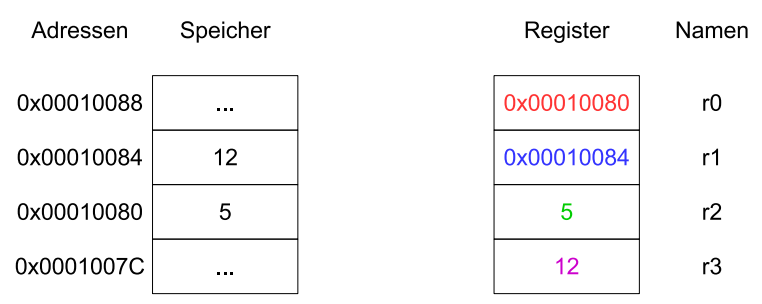
\includegraphics[width=12cm]{speicherBild.PNG}
                    \end{itemize}
            \end{itemize}
    \end{itemize}

\subsection{Datenfelder (Arrays)}
    \begin{itemize}
        \item \textbf{Eigenschaften}
            \begin{itemize}
                \item Datenfelder bestehen aus mehreren Worten 
                \item Nützlich um auf eine große Zahl von Daten gleichen Typs zuzugreifen
                \item Zugriff auf einzelne Elemente über Index
                \item[] 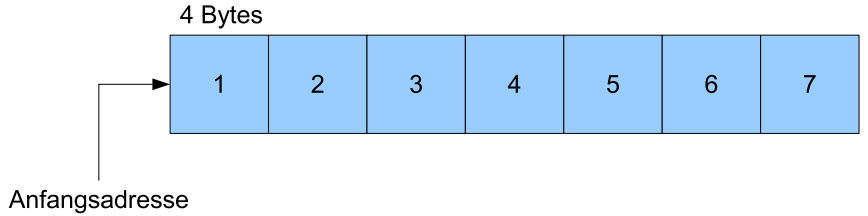
\includegraphics[width=12cm]{datenfeld1.PNG}
            \end{itemize} 

        \item \textbf{Verwendung von Arrays}
            \begin{itemize}
                \item[]
                    \begin{minipage}{0.35\textwidth}
                        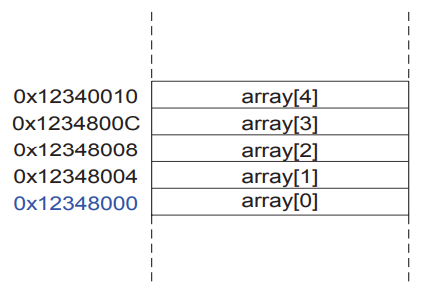
\includegraphics[width=6cm]{arraybsp.PNG}
                    \end{minipage}
                    \begin{minipage}{0.55\textwidth}
                        \begin{itemize}
                            \item Array mit 5 Elementen
                            \item Basisadresse: Adresse des ersten Elements (0x1234800)
                            \item Erster Schritt für Zugriff: Lade Basisadresse des Arrays in Register
                        \end{itemize}
                    \end{minipage}
                \item Beispiel:
                \item[]
                    \begin{minted}[autogobble]{c}
                    /* Umsetzung des folgenden C-Codes in Assembler */
                    int i;
                    int scores[200];
                    for (i = 0; i < 200; i = i + 1)
                        scores[i] = scores[i] + 10;
                    \end{minted}
                \item[]
                    \begin{minted}[autogobble]{c}
                    mov r0,#0x14000000  /* Speichern der Basisadresse des Arrays in r0 */
                    mov r1,#0           /* Verwendung als Zählervariable i */
                    LOOP:               
                    cmp r1,#200         /* i < 200 */
                    bge L3              /* Falls i > 200, Verlassen des Loops */
                    lsl r2,r1,#2        /* r2 = i * 4 -> Aufgrund des Offsets des Arrays von 4 */
                    ldr r3,[r0,r2]      /* Laden des Wertes aus Array / r3 = scores[i] */
                    add r3,r3,#10       /* r3 = scores[i] + 10 */
                    str r3,[r0,r2]      /* Zurückschreiben in Speicher / r3 Quellregister (nicht Ziel) */
                                        /* scores[i] = scores[i] + 10 */
                    add r1,r1,#1        /* i = i + 1 / Hochzählen der Laufvariable */
                    b LOOP              /* Wiederholen der Schleife */
                    L3:
                    ...
                    \end{minted}
            \end{itemize}
    \end{itemize}

\pagebreak

\subsection{Unterprogramme}
    \begin{itemize}
        \item \textbf{Einführung}
            \begin{itemize}
                \item Unterprogramme helfen bei der strukturierten Programmierung
                \item Betrachtung Hauptprogramm, in dem ein Teilprogramm an versch. Stellen ausgeführt werden soll
                \item Zwei Konzepte: Makrotechnik und Unterprogrammtechnik
            \end{itemize}

        \item \textbf{Makrotechnik}
            \begin{itemize}
                \item[]
                    \begin{minipage}{0.25\textwidth}
                        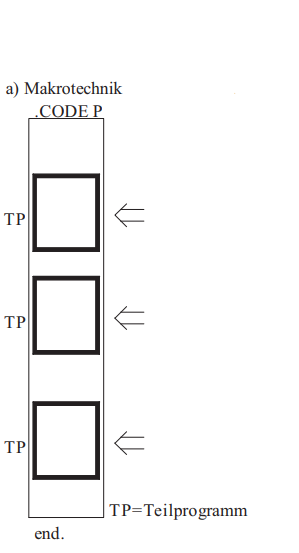
\includegraphics[width=3cm]{makrotechnik.PNG}
                    \end{minipage}
                    \begin{minipage}{0.65\textwidth}
                        \begin{itemize}
                            \item Teilprogramm wird, an benötigten Stellen, einkopiert
                            \item Zuordnung eines Namens für Teilprogramm (Makroname)
                            \item Nennung des Makronamens an besagter Stelle (Makroaufruf)
                        \end{itemize}
                    \end{minipage}
            \end{itemize}

        \item \textbf{Unterprogrammtechnik}
            \begin{itemize}
                \item[]
                    \begin{minipage}{0.25\textwidth}
                        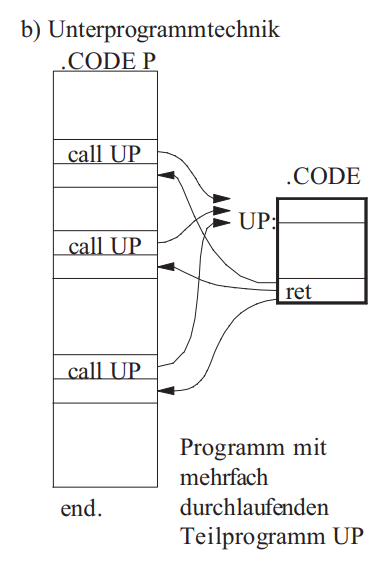
\includegraphics[width=5cm]{unterprogramm.PNG}
                    \end{minipage}
                    \begin{minipage}{0.65\textwidth}
                        \begin{itemize}
                            \item Teilprogramm nur einmal im Code vorhanden
                            \item Kennzeichnung durch Marke (Unterprogrammname)
                            \item Aufruf: Sprungbefehl + Marke 
                            \item Rückkehr in aufrufendes Programm nach Ausführung
                            \item[] $\Rightarrow$ durch Sprungbefehl auf Rückkehradresse
                            \item Rückkehradresse wird an anderer Stelle gespeichert
                            \item Beachten der Sichtbarkeit von Variablen (global vs lokal)
                        \end{itemize}
                    \end{minipage}
            \end{itemize}

\pagebreak

        \item \textbf{Funktions- und Prozeduraufruf}
            \begin{itemize}
                \item Aufrufer:
                    \begin{itemize}
                        \item Ursprung des Funktionsaufrufs
                        \item Übergibt Argumente (aktuale Parameter) an Aufgerufenen
                        \item Springt Aufgerufenen an
                    \end{itemize}

                \item Aufgerufener:
                    \begin{itemize}
                        \item Aufgerufene Funktion
                        \item Führt Funktion/Prozedur aus
                        \item Gibt Rückgabewert an Aufrufer zurück 
                        \item Darf keine Register oder Speicherstellen überschreiben, die im Aufrufer genutzt werden
                            \begin{itemize}
                                \item Beachten mit Sorgfalt und vorhandenem Konzept
                                \item Genutzte Register sollten gesichert werden, um danach wieder zu überschreiben
                            \end{itemize}
                    \end{itemize}
                
                \item Beispiel:
                    \begin{itemize}
                        \item[]
                            \begin{minted}[autogobble]{c}
                            /* Übersetzen des folgenden C-Codes in Assembler */
                            int main() {
                                int y;
                                y = diffofsums(14, 3, 4, 5); 
                            }

                            int diffofsums(int f, int g, int h, int i){ /* 4 formale Parameter */
                                int result;
                                result = (f + g) - (h + i);
                                return result;
                            }
                            \end{minted}
                        \item[]
                        \item[]
                            \begin{minted}[autogobble]{c}
                            /* ASSEMBLER */
                            /* r4 = y */
                            main:
                            mov r0,#14      /* Argument 0 = 14 */
                            mov r1,#3       /* Argument 1 = 3 */
                            mov r2,#4       /* Argument 2 = 4 */
                            mov r3,#5       /* Argument 3 = 5 */
                            bl diffofsums   /* Funktionsaufruf / bl: branch and link */
                            /* Schreibt die Rückkehradresse des folgenden Befehls mov in link register (r14) */
                            mov r4,r0       /* y = Rückgabewert */
                            -------------
                            diffofsums:
                            add r8,r0,r1    /* Überschreiben von r8 / Kein Sichern der Werte vorher */
                            add r9,r2,r3    /* Selbiges gilt für r9 */
                            sub r4,r8,r9
                            mov r0,r4       /* Ablegen von Rückgabewert in r0 (return value register) */
                            mov pc,lr       /* Übergabe der Rückkehradresse an Program Counter */
                            /* Program Counter führt dann den nächsten Befehl (mov r4,r0) aus */
                            \end{minted}
                    \end{itemize}
            \end{itemize}
    \end{itemize}
        
\pagebreak

\subsection{Stack}
    \begin{itemize}
        \item \textbf{Eigenschaften des Stacks}
            \begin{itemize}
                \item Speicher für temporäres Zwischenspeichern von Werten
                \item LIFO-Konzept (\string"last in, first out"\string)
                \item Dehnt sich aus, falls mehr Daten gespeichert werden müssen
                \item Zieht sich zusammen, wenn weniger Daten gespeichert werden müssen
                \item Wächst bei ARM nach unten (von hohen zu niedrigen Adressen)
                \item Verwendung des \texttt{Stackpointers sp (r13)}
                \item \texttt{StackPointer} zeigt auf letztes auf dem Stack abgelegtes Element
            \end{itemize}

        \item \textbf{Verwendung des Stacks bei Unterprogrammen}
            \begin{itemize}
                \item Beispiel \texttt{diffofsums}:
                    \begin{itemize}
                        \item[]
                            \begin{minted}[autogobble]{c} 
                            diffofsums:
                            add r8, r0, r1
                            add r9, r2, r3
                            sub r4, r8, r9
                            mov r0, r4      /* Rueckgabewert in r0 */
                            mov pc, lr      /* Ruecksprung zum Aufrufer */
                            \end{minted}
                        \item[]
                        \item Problem hier: \texttt{diffofsums} überschreibt r8, r9, r4 
                        \item Unterprogramme dürfen aber keine unbeabsichtigten Seiteneffekte haben
                        \item Vorherige Werte in r8, r9 und r4 gehen hierbei aber verloren
                    \end{itemize}

                \item Lösung: Register auf Stack Zwischenspeichern
                    \begin{itemize}
                        \item[]
                            \begin{minted}[autogobble]{c}
                            diffofsums:
                            sub sp, sp, #12     /* Speicher auf Stack reservieren (3 Adressen "abziehen") */
                            str r9, [sp, #8]    /* Speichern an oberster freier Stelle im Stack */
                            str r8, [sp, #4]
                            str r4, [sp]        /* Speichern an unterster freier Stelle im Stack */
                            /* Abspeichern der Werte in Benutzungsreihenfolge hier als Konvention */
                            add r8, r0, r1      /* Berechnungen durchführen */
                            add r9, r2, r3
                            sub r4, r8, r9
                            mov r0, r4          /* Rückgabewert in r0 */

                            /* Wiederherstellen der Werte nun in umgekehrter Reihenfolge */
                            ldr r4, [sp]        /* Wiederherstellen von r4 */
                            ldr r8, [sp, #4]    /* Wiederherstellen von r8 */
                            ldr r9, [sp, #8]    /* Wiederherstellen von r9 */
                            add sp, sp, #12     /* Freigabe von Speicher auf dem Stack */

                            mov pc, lr          /* Rücksprung zum Aufrufer */
                            \end{minted}
                        \item[]
                        \item[] 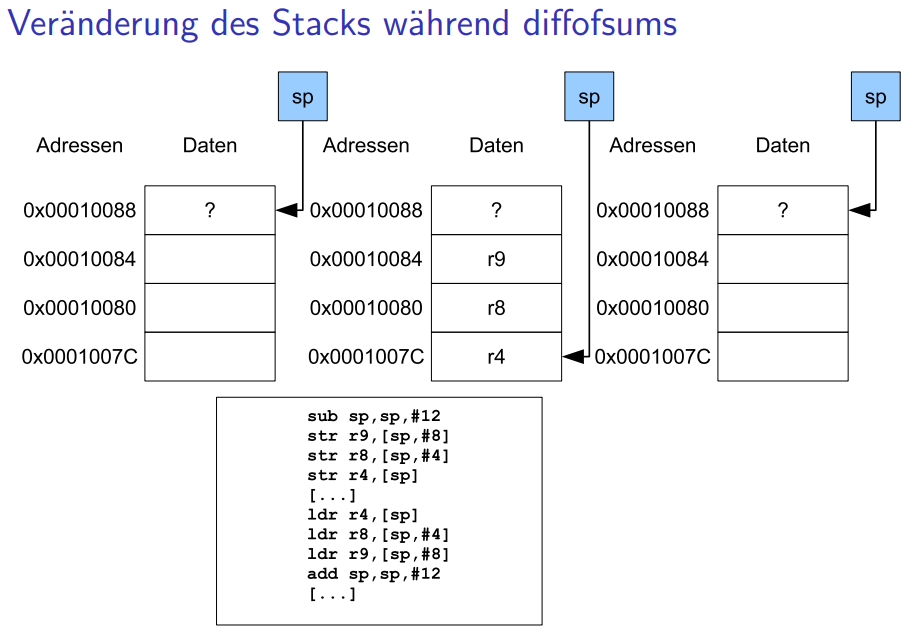
\includegraphics[width = 8cm]{stackGrafik.png}
                    \end{itemize}

                \item Verwendung des Stacks auch bei Unterprogrammaufrufen
                    \begin{itemize}
                        \item Das \texttt{LinkRegister} muss vor Unterprogrammaufrufen gesichert werden
                        \item[]
                            \begin{minted}[autogobble]{c}
                            main:
                            ...
                            push {lr}       /* push ist hier nur eine Pseudoinstruktion für str */
                            bl diffofsums   /* Das LinkRegister wird beim Programmaufruf verändert */
                            ...
                            pop {lr}        /* pop ist hier die Pseudoinstruktion für ldr */
                            bx lr       
                            \end{minted}
                        \item[]
                        \item \texttt{push} und \texttt{pop} sind auch mit Operandenliste möglich
                            \begin{itemize}
                                \item \texttt{push \{r9, r8, r4\}}
                                \item Allerdings muss hierbei das \string"poppen\string" in umgekehrter Reihenfolge beachtet werden
                            \end{itemize}
                    \end{itemize}
            \end{itemize}
    \end{itemize}

\subsection{Rekursion}
    \begin{itemize}
        \item \textbf{Graphische Betrachtung}
            \begin{itemize}
                \item[] 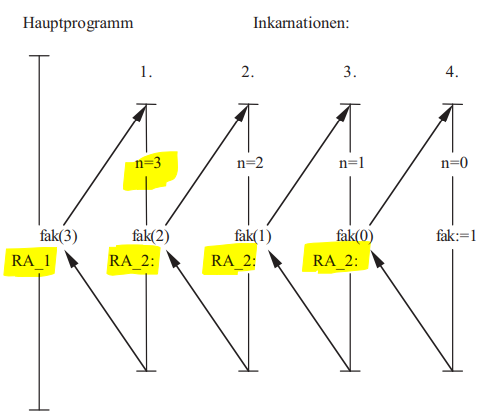
\includegraphics[width=8cm]{rekursion.PNG}
                \item[] 
                \item Inkarnation: Ablauf eines Unterprogrammes
                \item Zwei verschiedene Rückkehradressen:
                    \begin{itemize}
                        \item \textbf{RA\_1}: Adresse im Hauptprogramm
                        \item \textbf{RA\_2}: Adresse im Unterprogramm
                        \item \textbf{RA\_2} ist immer diesselbe Adresse, da immer selber Code
                    \end{itemize} 
            \end{itemize}

\pagebreak

        \item \textbf{Code: Fakultätsberechnung}
            \begin{itemize}
                \item[]
                    \begin{minted}[autogobble]{c}
                    .global main

                    main:                       /* Hauptprogramm */
                            push{lr}            /* Sicherung lr */
                            mov r0, #3          /* fak von 3 */
                            bl fak              /* Aufruf von fak */
                    RA_1:   mov r4, r0          /* RA_1 ist hier kein sinnvoller Code, nur für Adressen hier */
                            mov r0, r4
                            pop {lr}
                            bx lr
                    
                    fak:    sub sp, sp, #8      /* Stackspeicher reservieren */
                            str r0, [sp, #4]    /* Sichern von r0 */
                            str lr, [sp]        /* Sichern lr */
                            cmp r0, #1          /* Überprüfung Rekursionsende */
                            blt else            
                            sub r0, r0, #1      /* n = n - 1 */
                            bl fak              /* Funktionsaufruf */
                    RA_2:   ldr r1, [sp, #4]    /* Laden von n */
                            mul r0, r1, r0      /* fak (n-1) * n */
                    fin:    ldr lr, [sp]        /* Laden Rückkehradresse */
                            add sp, sp, #8      /* Freigabe Stackspeicher */
                            bx lr
                    else:   mov r0, #1          /* Rekursionsanker */
                            b fin
                    \end{minted}
                \item[]
                \item Aufrufer:
                    \begin{itemize}
                        \item Lege Aufrufparameter in Register oder auf Stack ab 
                        \item Sichere notwendige Register auf dem Stack (lr)
                        \item Rufe Unterprogramm auf (bl)
                        \item Stelle gesicherte Register wieder her (lr)
                        \item Verwendung von Rückgabewert
                    \end{itemize}
                
                \item Aufgerufener:
                    \begin{itemize}
                        \item Sichere zu erhaltende Register auf dem Stack 
                        \item Führe Unterprogrammrechnung aus
                        \item Rückgabewert in r0 legen
                        \item Wiederherstellen der gesicherten Register
                        \item Rücksprung zum Aufrufer
                    \end{itemize}
            \end{itemize}
    \end{itemize}

\pagebreak

\subsection{Compilieren, Assemblieren und Linken}
    \begin{itemize}
        \item \textbf{Optimierungseinstellungen}
            \begin{itemize}
                \item Generieren des Assemblercodes mithilfe von \texttt{gcc -S code.c} führt zu viel \string"unnötigem"\string Code
                \item z.B. das Speichern von immediate Values auf dem Stack etc
                \item Optimierungsstufen (\texttt{gcc -S -O1 code.c}) erzeugen meist \string"weniger"\string Code
                \item Die Übersetzung eines Programmes kann also viele verschiedene Ergebnisse haben
                \item Außerdem werden nicht unbedingt alle Elemente einer Hochsprache in Assembler sichtbar
            \end{itemize}

        \item \textbf{OpenMP (Einschub)}
            \begin{itemize}
                \item Threadparalleles Arbeiten auf Rechnersystemene mit gemeinsamen Adressraum
                \item Gut geeignet für Multicore-Architekturen
                \item Programm verzweigt automatisch bei parallel-ausführbarem Code in zusätzliche Threads
                \item Am Schluss werden diese Threads wieder zu einem einzelnen zusammengeführt
                \item \textbf{Fork-Join-Programmiermodell}
                \item Verwenden in der Praxis:
                    \begin{itemize}
                        \item Einbinden von \texttt{\#include<omp.h>}
                        \item Compileraufruf: \texttt{gcc - fopenmp name.c}
                        \item Setzen Umgebungsvariable für Threadanzahl: \texttt{OMP\_NUM\_THREADS=2}
                    \end{itemize}
                \item Programme lassen sich aber eher selten sehr gut parallelisieren
            \end{itemize}

        \item \textbf{Assemblerprogramm}
            \begin{itemize}
                \item Definition: 
                    \begin{itemize}
                        \item Programm, das die Aufgabe hat, Assemblerbefehle in Maschinencode zu transformieren
                        \item symbolischen Namen (Labels) Maschinenadressen zuzuweisen
                        \item Erzeugung einer oder mehrerer Objektdateien
                    \end{itemize}

                \item \textbf{Crossassembler}
                    \begin{itemize}
                        \item Assembler läuft auf Rechnersystem X, generiert aber Maschinencode für Platform Y
                        \item Verwendung im Bereich der Embedded Systems
                    \end{itemize}
                
                \item \textbf{Disassembler}
                    \begin{itemize}
                        \item Übersetzung von Maschinencode in Assemblersprache
                        \item Verlust von Kommentaren und symbolischen Namen
                    \end{itemize}
            \end{itemize}

        \item \textbf{Schrittweiser Assembliervorgang}
            \begin{itemize}
                \item 1. Schritt:
                    \begin{itemize}
                        \item Auffinden von Speicherposition mit Marken (Beziehung zwischen Adresse und Namen bekannt)
                        \item Übersetzung jedes Assemblerbefehls durch OPCodes, Register und Marken in legale Instruktion
                    \end{itemize}
                \item 2. Schritt
                    \begin{itemize}
                        \item Erzeugung einer oder mehrerer Objektdateien
                        \item Enthalten Maschinencode, Daten, Verwaltungsinformationen
                        \item Jedoch meist nicht ausführbar (Verweise auf andere Funktionen etc.)
                    \end{itemize}
                \item Probleme beim 1. Schritt
                    \begin{itemize}
                        \item Nutzen von Marken, bevor sie definiert sind (Unbekannte Adressen)
                        \item Lösung: \textbf{Two-Pass}
                            \begin{itemize}
                                \item Assembler macht 2 Läufe über das Programm
                                \item 1. Lauf: Zuordnen von Maschinenadressen
                                \item 2. Lauf: Erzeugen der Codes
                            \end{itemize}
                    \end{itemize}
\pagebreak
                \item Probleme beim 2. Schritt (Erzeugen des Objektdatei)
                    \begin{itemize}
                        \item 1. Fall:
                            \begin{itemize}
                                \item Assembler verwendet \textbf{absolute} Adreessen und eine Objektdatei
                                \item Laden unmittelbar möglich, Speicherort muss jedoch vorher bekannt sein
                                \item Nachteil: Verschieben des Programms nicht möglich
                            \end{itemize}

                        \item 2. Fall:
                            \begin{itemize}
                                \item Assembler verwendet \textbf{relative} Adressen und ggf. mehrere Programm-Segmente als Eingabe
                                \item Assembler Ausgabe: $\geq$ 1 Objekt-Dateien
                                \item Adressen werden relativ zu Objektdateien vergeben
                                \item Deswegen sind weitere Transformationsschritte notwendig (Binder/Linker/Lader)
                            \end{itemize}
                    \end{itemize}
            \end{itemize}

        \item \textbf{Aufbau eines Objekt-Programms}
            \begin{itemize}
                \item Verschiedene Arten von Objekt-Programmen:
                    \begin{itemize}
                        \item Relocatable (verschiebbare) Object Files:
                            \begin{itemize}
                                \item[] Enthalten binären Code und Daten in einer Form, die mit anderen 
                                        verschiebbaren \\ Objekt-Files zu einem ausführbaren Objekt-File zusammengefügt werden können. \\
                                        Diese Files werden in der Regel generiert.
                            \end{itemize}
                        \item Executable Object Files:
                            \begin{itemize}
                                \item[] Enthalten binären Code und Daten in einer Form, die direkt in den Speicher kopiert
                                        und ausgeführt werden kann. 
                            \end{itemize}
                        \item Shared Object Files:
                            \begin{itemize}
                                \item[] Spezieller Typ von Relocatable Object Files, welche in den Speicher geladen werden können
                                        und dynamisch mit anderen Object-Files zusammengeführt werden können.
                            \end{itemize}
                    \end{itemize}

                \item Aufbau eines ELF relocatable object files
                    \begin{itemize}
                        \item[]
                            \begin{minipage}{0.35\textwidth}
                                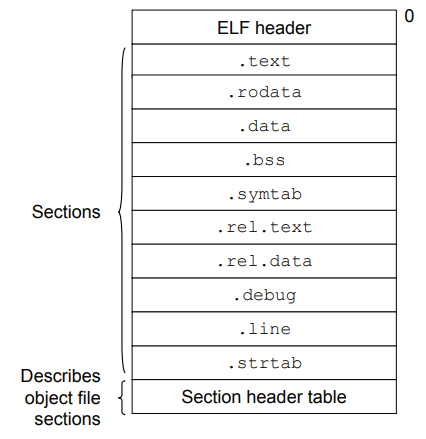
\includegraphics[width=7cm]{elfheader.PNG}
                            \end{minipage}
                            \begin{minipage}{0.55\textwidth}
                                \vspace{-2cm}
                                \begin{itemize}
                                    \item ELF: Ein Format dieser Files
                                    \item Beginnt mit 16-Byte Sequenz
                                    \item Informationen über Wortgrö\ss e, Byte-Ordering,..
                                    \item .text: Maschinencode des compilierten Programms
                                    \item .data: Initialisierte globale Variablen
                                    \item etc.
                                \end{itemize}
                            \end{minipage}

                        \item[]
                        \item Beispiel einer ELF-Header-File (16 Bytes)
                            \begin{itemize}
                                \item \texttt{as -o prog.o prog.s} (Übersetzung eines C-Programms)
                                \item \texttt{readelf -h prog.o} (Lesen ELF-Header / -h für Header) 
                                \item[] 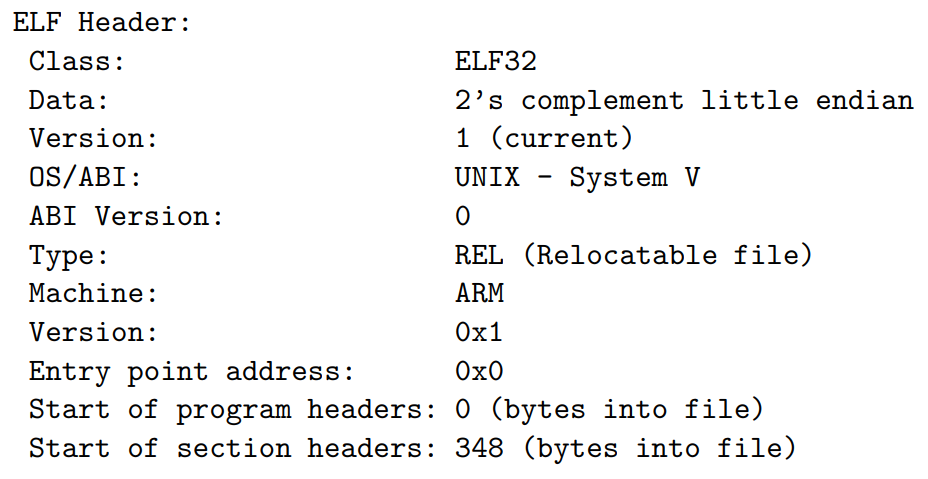
\includegraphics[width=9cm]{elfheaderbsp.PNG}
                                \item[]
                                \item \texttt{readelf -a prog.i} (Übersicht über wichtigsten Einträge)
                                \item \texttt{objdump -S prog.o} (Rückgabe des Maschinencodes)
                                \item[] 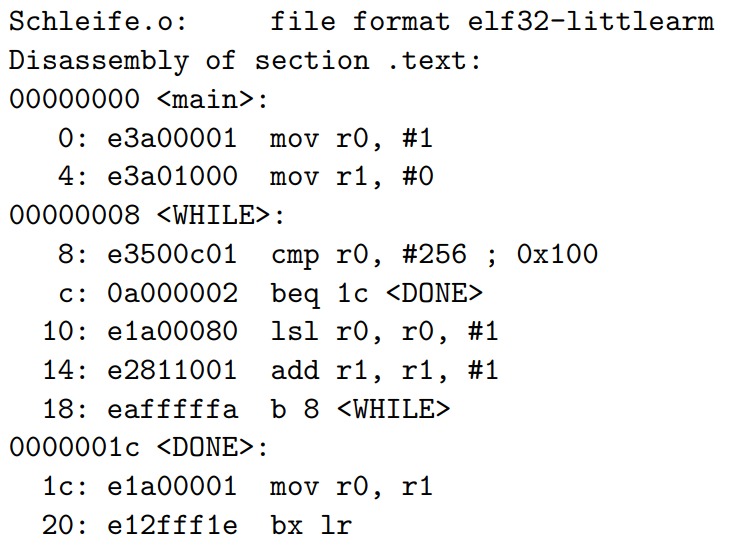
\includegraphics[width=9cm]{objdump.PNG}
                                \item Links ist der Maschinencode mit 8 Byte (32 Bit) in Hexa zu sehen 
                            \end{itemize}
                    \end{itemize}
            \end{itemize}

        \item \textbf{Binder/Linker und Lader}
            \begin{itemize}
                \item Definition Binder/Linker
                    \begin{itemize}
                        \item Erzeugung eines ausführbaren Objektprogramms aus einzelnen verschiebbaren Objekt-Files
                        \item Hierzu auflösen der offenen exteren Referenzen
                    \end{itemize}
                \item Definition Lader
                    \begin{itemize}
                        \item Systemprogramm, das die Objektprogramme in den Speicher lädt und die Ausführung anstö\ss t
                        \item Kopieren des Objektprogrammes in den Speicher
                        \item Verschiedene Arten des Ladevorgangs:
                            \begin{itemize}
                                \item absolutes Laden (absolute loading)
                                \item relatives Laden (relocatable loading)
                                \item dynamisches Laden zur Laufzeit (dynamic run-time loading)
                            \end{itemize}
                    \end{itemize}
            \end{itemize}

        \item \textbf{Laufzeitanalyse von C-Programmen}
            \begin{itemize}
                \item Erinnerung: Operationen auf den Registern sind schneller als Operationen auf Hauptspeicher
                \item Möglichkeit des Programm Profiling hier:
                    \begin{itemize}
                        \item Hauptprogramm, das zwei Funktionen (eine iterativ, andere rekursiv) aufruft
                        \item \texttt{gcc} kann hier bei der Bestimmung der Laufzeit weiterhelfen
                        \item \texttt{gcc -pg -o function\_fak function\_fak.c} (-pg ist ein run-time flag)
                        \item Danach Aufruf des Programms (dauert etwas länger)
                        \item \texttt{gprof function\_fak gmon.out > analysis.txt} (Wertet die Profile-Datei aus)
                        \item Diese splittet die Zeit der Unterprogramme auf und zeigt die Laufzeiten an
                    \end{itemize}
            \end{itemize}
    \end{itemize}

\pagebreak

\section{Mikroarchitekturen von Rechnersystemen}
\subsection{Begrifflichkeiten und Grundlagen}
    \begin{itemize}
        \item \textbf{Drei Phasen der Befehlsausführung}
            \begin{itemize}
                \item Befehle, als auch Daten stehen im Speicher
                \item \textit{Befehlsholphase:} Prozessor liest die Befehle aus dem Speicher
                \item \textit{Befehlsdekodierung:} Dekodierung des Befehls, nachdem dieser in ein Register geholt wurde
                \item \textit{Befehlsausführung:} Ausführung des Befehls, danach Holen des nächsten Befehls
            \end{itemize}

        \item \textbf{Takt/Taktfrequenz}
            \begin{itemize}
                \item Gemeinsame Zeitbasis der Komponenten eines Rechnersystems: Takt
                \item Beim Takt handelt es sich um ein Rechtecksignal
                \item Dient der Synchronisation der Komponenten eines Rechnersystems
                \item Taktfrequenz: $f = \frac{1}{T}$
                \item Je höher Taktfrequenz, desto schneller werden Daten verarbeitet
                \item Leistungssteigerung durch Erhöhen der Taktfrequenz (CMOS: $P = U^2 \cdot f \cdot C_l$)
            \end{itemize}

        \item \textbf{Terminologie}
            \begin{itemize}
                \item \textit{ISA}: instruction set architecture (Menge der verfügbaren Befehle)
                \item \textit{RISC}: reduced instruction set computer (kleine ISA)
                \item \textit{CISC}: complex instruction set computer (aufwendige ISA)
                \item \textit{SIMD}: single instruction multiple data (paralleles Arbeiten)
                \item \textit{VLIW}: verly long instruction word (static multi-issue)
                \item \textit{$\mu$arch}: microarchitecture (Hardware, die ISA abarbeitet - ISA Implementierung)
                    \begin{itemize}
                        \item \textit{IPC}: Anzahl der Befehle pro Zyklus
                        \item \textit{ILP}: Pipelining für Parallelismus
                        \item Sprungvorhersagen,... etc
                    \end{itemize}
            \end{itemize}
    \end{itemize}

\subsection{Analyse der Rechenleistung}
    \begin{itemize}
        \item \textbf{Mikroarchitektur}
            \begin{itemize}
                \item \textit{Mikroarchitektur:} Hardware-Implementierung einer Architektur
                \item \textit{Datenpfad:} Verbindet funktionale Blöcke (Speicher/Prozessor)
                \item \textit{Kontrollpfad:} Steuersignale/Steuerwerk
                \item \textit{Eintakt-Implementierung:} Jeder Befehl wird in einem Takt ausgeführt
                \item \textit{Mehrtakt-Implementierung:} Jeder Befehl wird in Teilschritte zerlegt
                \item \textit{Pipeline-Implementierung:} Teilschritte + Parallele Ausführung der Teilschritte
            \end{itemize}
        \item \textbf{Rechenleistung eines Prozessors}
            \begin{itemize}
                \item Ausführungszeit eines Programms
                \item[] $\Rightarrow$ $Ausfuehrungszeit$ = (\#$Instruktionen$) $\cdot$ ($\frac{Takte}{Instruktion}$) $\cdot$ ($\frac{Sekunden}{Takt})$
                \item \texttt{CPI}: Takte/Instruktion
                \item \texttt{Taktperiode}: Sekunden/Takt
                \item \texttt{IPC}: 1/CPI = Instruktionen/Takt
            \end{itemize}
\pagebreak
        \item \textbf{Mikroarchitektur ARM}
            \begin{itemize}
                \item \textit{Befehlsmenge:} (ldr, add, sub etc)
                \item \textit{Architekturzustand:} Sichtbare Daten auf Ebene der Architektur
                \item Sichtbare Daten bestimmen den Zustand (Program Counter, 16 Register, etc)
            \end{itemize}
        \item \textbf{Elemente des Architekturzustands}
            \begin{itemize}
                \item[] 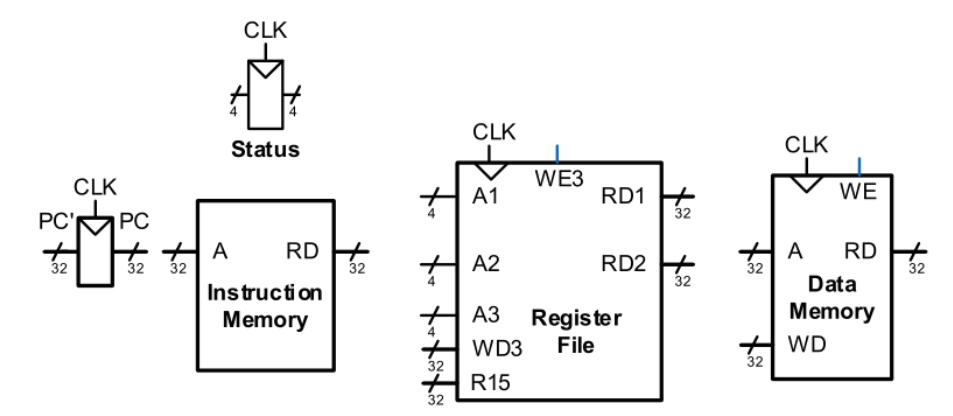
\includegraphics[width=10cm]{architekturzustand.PNG}
                \item \textit{Register File}
                    \begin{itemize}
                        \item A1,A2,.. - \textit{Registeradresse} (4 Bit $\rightarrow$ 16 Möglichkeiten)
                        \item RD1,RD2,.. - \textit{Register Data} (Ausgabedaten)
                        \item WD3 - \textit{Write Data 3} (Eingabedaten)
                    \end{itemize}
                \item \textit{Status}
                    \begin{itemize}
                        \item Gibt Flags an mit 4 Bits (Sign, Zero, Overvlow, Carry)
                    \end{itemize}
                \item \textit{Program Counter (PC)}
                \item \textit{Instruction Memory}
                    \begin{itemize}
                        \item A - \textit{Adressen}
                        \item RD - \textit{Read Data} (Instruktionen)
                    \end{itemize}
                \item \textit{Data Memory}
                    \begin{itemize}
                        \item WE - \textit{Write Enable} (Benötigt für Schreibprozesse - Steuersignal)
                    \end{itemize}
            \end{itemize}

        \item \textbf{Von-Neumann-/Harvard-Architektur}
            \begin{itemize}
                \item Von-Neumann: gemeinsamer Speicher für Befehle und Daten
                \item Harvard-Architektur: Befehlsspeicher und Datenspeicher sind getrennt
                \item Verhalten des Speichers: Asynchrones Lesen möglich, jedoch nur Synchrones Schreiben
            \end{itemize}

        \item \textbf{Vorgehensweise und Bitfelder eines Befehls}
            \begin{itemize}
                \item Hier: Befehl \texttt{ldr}
                \item Allgemein: \texttt{ldr Rd, [Rn, imm12]} (imm12: immediate value - 12 Bit)
                \item[] 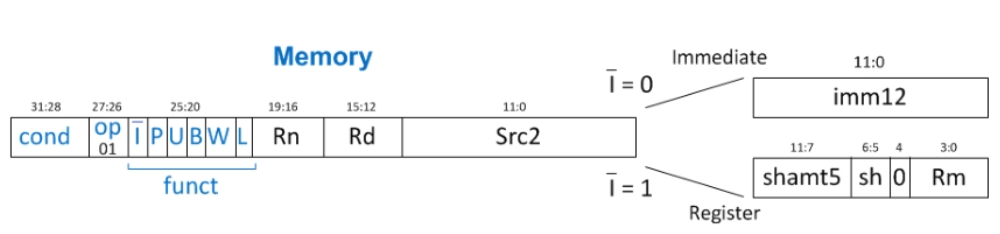
\includegraphics[width=10cm]{befehlsBitfeld.PNG}
                \item 32 Bit Länge -> z.B.: E13A0110 (In Hexa)
                \item \textbf{Rd}: Adresse register destination
                \item Ganz hinten entweder Register oder Direktwert (festgelegt durch \textbf{I})
                \item Vorne: Conditions für die Ausführung (möglich für \textit{jeden} Befehl)
            \end{itemize}
    \end{itemize}

\subsection{Eintakt-Prozessor}
    \begin{itemize}
        \item \textbf{Phasen der Befehlsausführung}
            \begin{itemize}
                \item[] 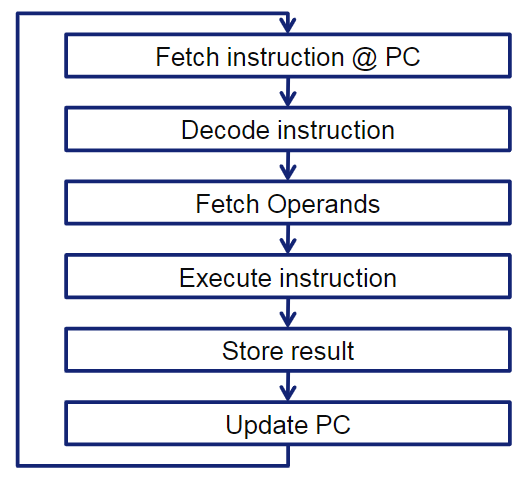
\includegraphics[width=6cm]{phasenBefehl.PNG}
            \end{itemize}

        \item \textbf{Ablauf der Befehlsausführung anhand eines Eintaktprozessors}
            \begin{itemize}
                \item[]
                    \begin{minipage}{0.45\textwidth}
                        \textit{1. Befehl holen} \\
                        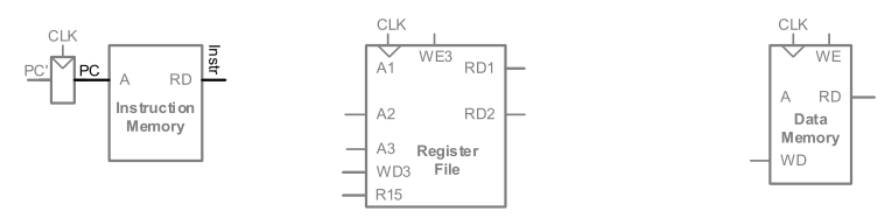
\includegraphics[width=7cm]{ep1.PNG}
                    \end{minipage}
                    \begin{minipage}{0.45\textwidth}
                        \textit{2.Lesen der Quelloperanden vom Registerfeld} \\
                        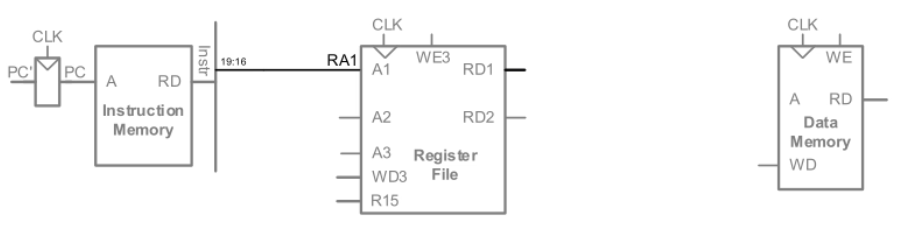
\includegraphics[width=7cm]{ep2.PNG}
                    \end{minipage}
                \item[]
                    \begin{minipage}{0.45\textwidth}
                        \textit{3. Erweiterung Direktwert (32 Bit)} \\
                        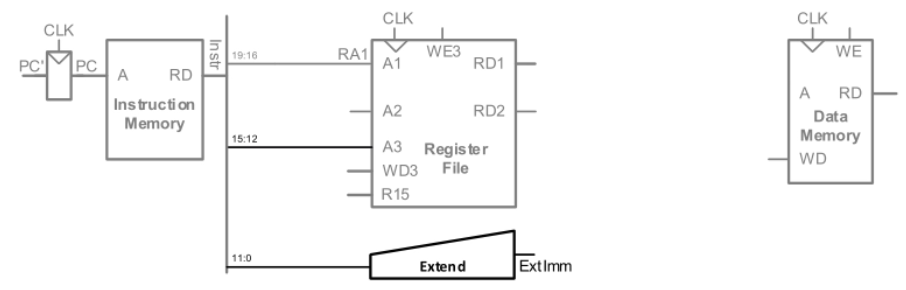
\includegraphics[width=7cm]{ep3.PNG}
                    \end{minipage}
                    \begin{minipage}{0.45\textwidth}
                        \textit{4. Berechnung der Speicheradresse} \\
                        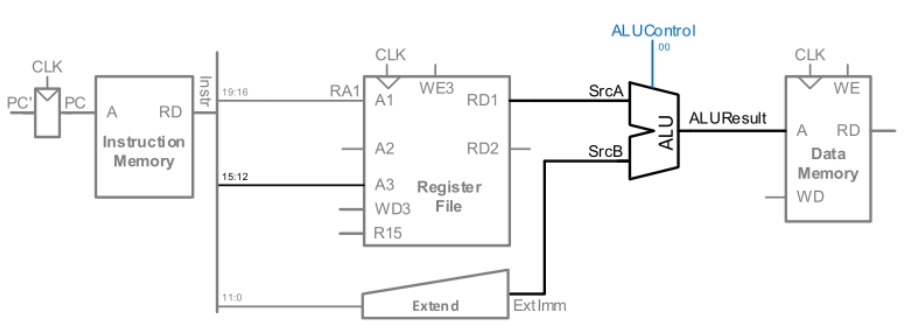
\includegraphics[width=7cm]{ep4.PNG}
                    \end{minipage}
                \item[]
                    \begin{minipage}{0.45\textwidth}
                        \textit{5. Lesen aus Speicher und Schreiber in Register} \\
                        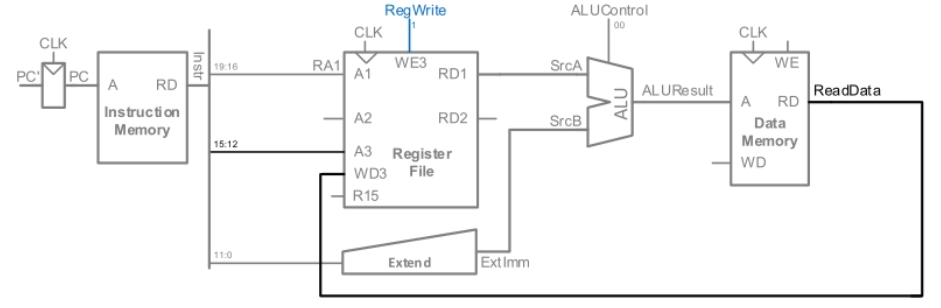
\includegraphics[width=7cm]{ep5.PNG}
                    \end{minipage}
                    \begin{minipage}{0.45\textwidth}
                        \textit{6. Berechnung der nächsten Befehladresse} \\
                        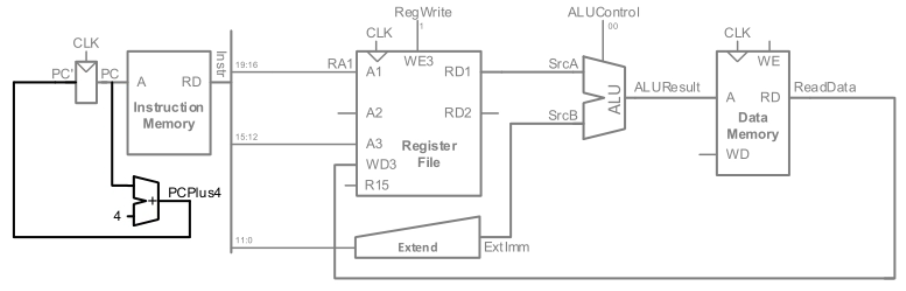
\includegraphics[width=7cm]{ep6.PNG}
                    \end{minipage}
            \end{itemize}

        \item \textbf{Befehl str}
            \begin{itemize}
                \item \texttt{STR Rd, [Rn, imm12]} (Rd hier Quellregister nicht Ziel - Rd nach Speicher schreiben)
                \item Erweiterung des Datenpfades zur Realisierung von \texttt{str}
                \item Schreibe DAtum vom registerfeld in den Datenspeicher
                \item[] 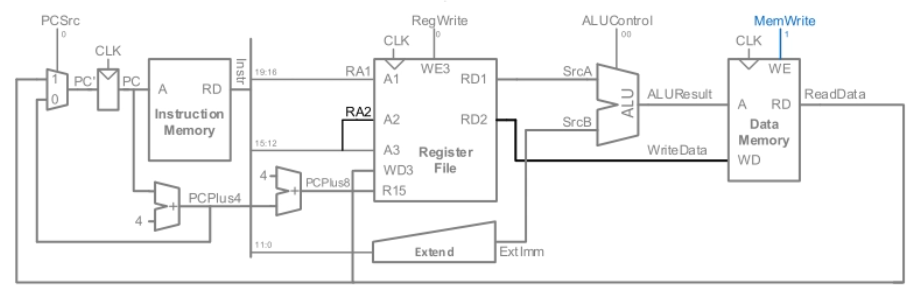
\includegraphics[width=10cm]{estr.PNG}
            \end{itemize}

\pagebreak
        
        \item \textbf{Arithmetische und logische Befehle}
            \begin{itemize}
                \item \texttt{ADD Rd, Rn, imm8}
                \item[] 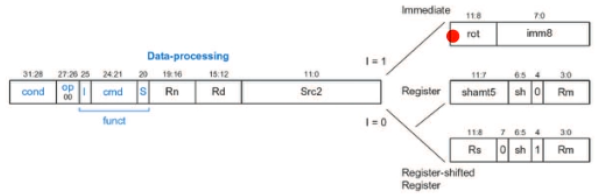
\includegraphics[width=8cm]{ep8.PNG}
                \item \textbf{\textit{immediate Src2} (Src2 hier als Direktwert)}
                \item[] $\Rightarrow$ Steuersignal \textit{ImmSrc} regelt um wieviele Bits erweitert wird
                \item[] $\Rightarrow$ 0: Erweiterung um 24 Bit (ALU-Befehle) | 1: Erweiterung um 20 Bit (ldr,str Befehle)
                \item[] $\Rightarrow$ Erweiterung um Multiplexer 
                \item[] $\Rightarrow$ Schreibe ALUResult in Registerfeld statt Speicher (je nach Multiplexer)
                \item[] 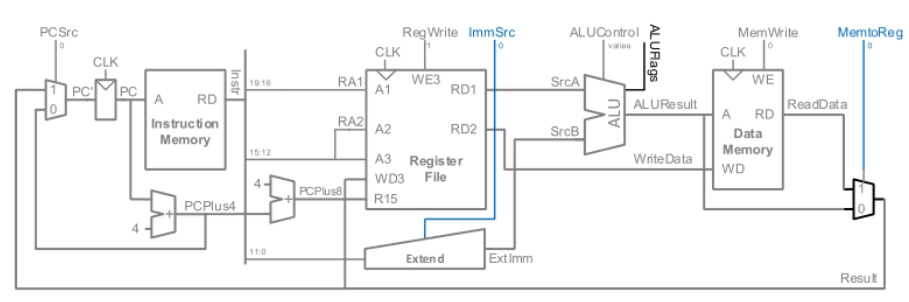
\includegraphics[width=10cm]{ep7.PNG}
                \item \textbf{\textit{Register Src2} (Src2 hier als Register)}
                \item[] $\Rightarrow$ Multiplexer vor Register File und nach Extend
                \item[] 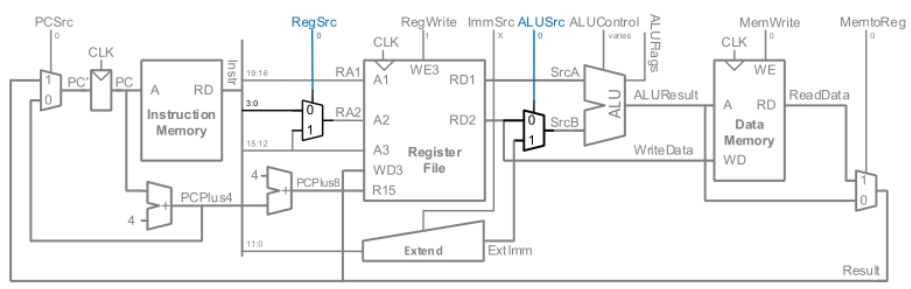
\includegraphics[width=10cm]{ep9.PNG}
            \end{itemize}

        \item \textbf{Arithmetisch Logische Einheit}
            \begin{itemize}
                \item[] 
                    \begin{minipage}{0.5\textwidth}
                        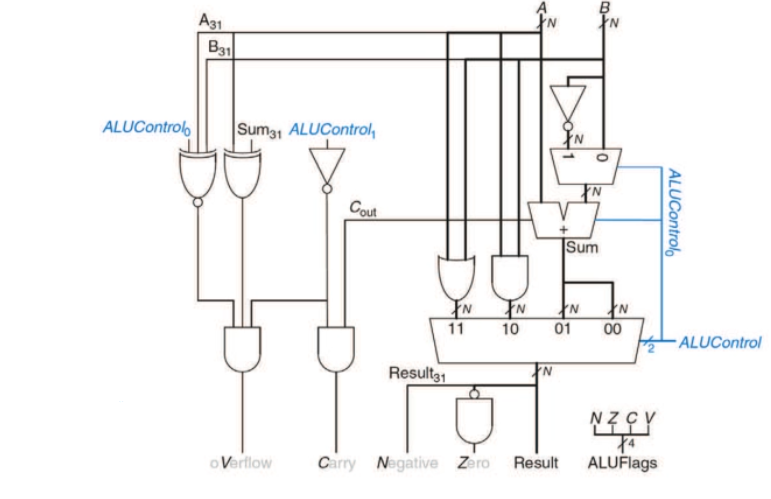
\includegraphics[width=8cm]{alu.PNG}
                    \end{minipage}
                    \begin{minipage}{0.4\textwidth}
                        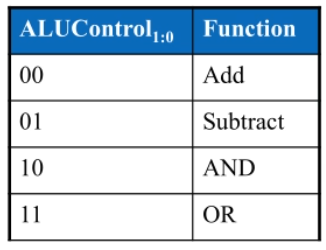
\includegraphics[width=6cm]{aluC.PNG}
                    \end{minipage}
            \end{itemize}

        \item \textbf{Sprungbefehl b}
            \begin{itemize}
                \item Berechnen der Sprungadresse
                \item BTA = (ExtImm) + (PC + 8)
                \item ExtImm = Imm24 << 2 inkl. Vorzeichenerweiterung+
                \item[] 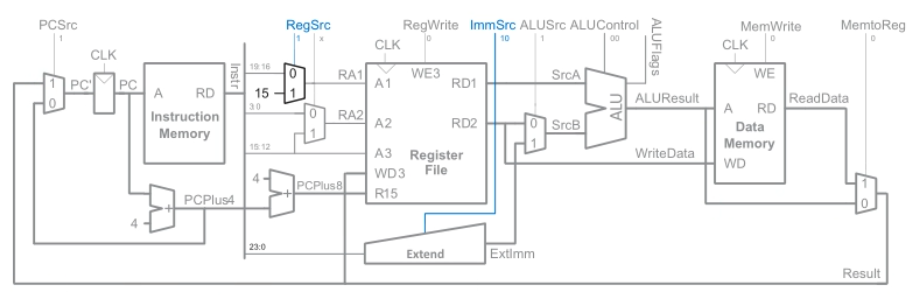
\includegraphics[width=10cm]{ep10.PNG}
            \end{itemize}

        \item \textbf{ExtImm}
            \begin{itemize}
                \item Unterschiedliche Funktionen werden benötigt
                \item Erweiterung der Werte auf 32 Bit wird benötigt
                \item[] 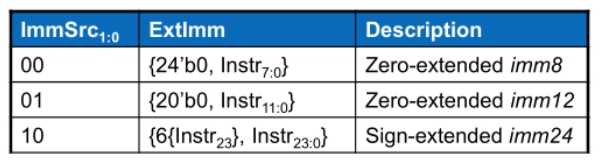
\includegraphics[width=8cm]{ep11.PNG}
                \item[] 6\{Instr$_{23}$\} $\rightarrow$ Erstes Bit 6x (Sprungbefehl)  
            \end{itemize}

        \item \textbf{Kontrolleinheit}
            \begin{itemize}
                \item[] 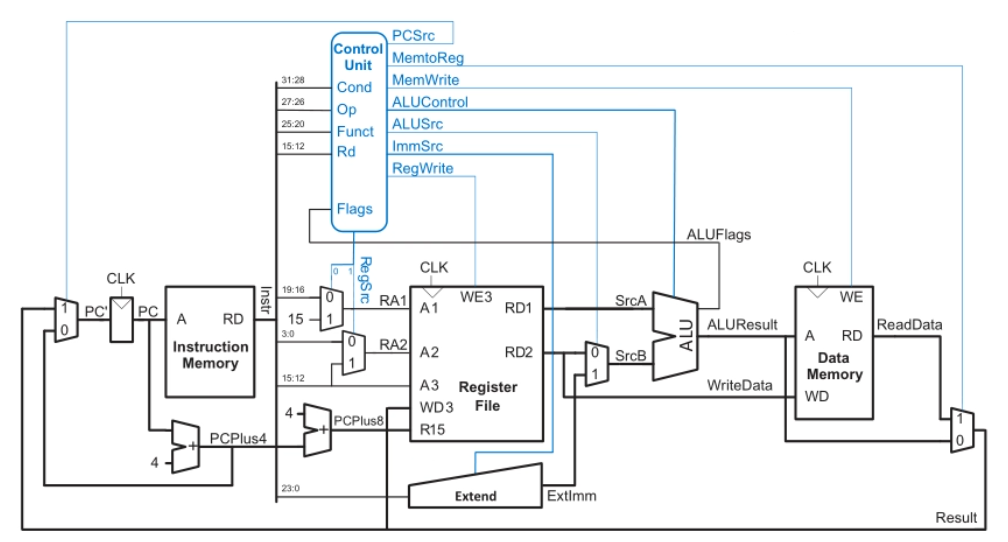
\includegraphics[width=10cm]{ep12.PNG}
                \item[]
                    \begin{minipage}{0.4\textwidth}
                        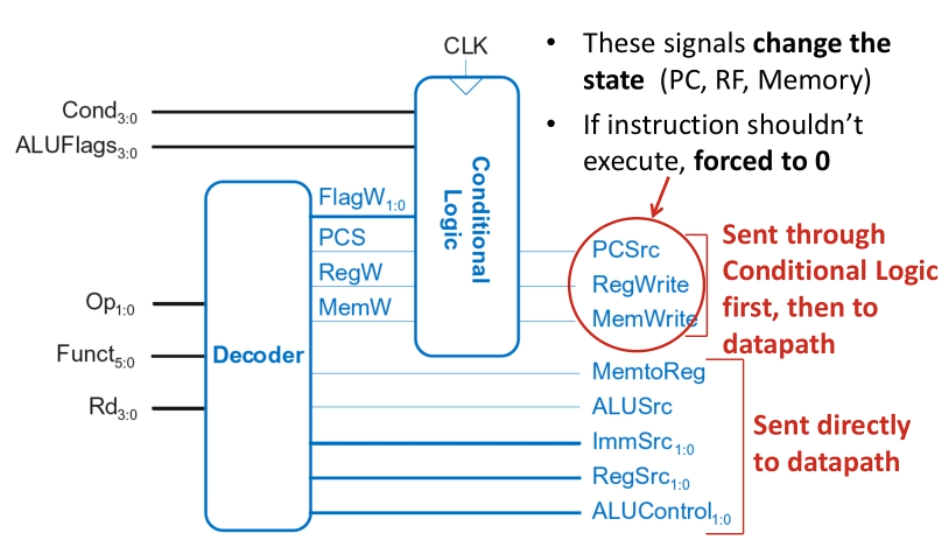
\includegraphics[width=7cm]{ep13.PNG}
                    \end{minipage}
                    \begin{minipage}{0.45\textwidth}
                        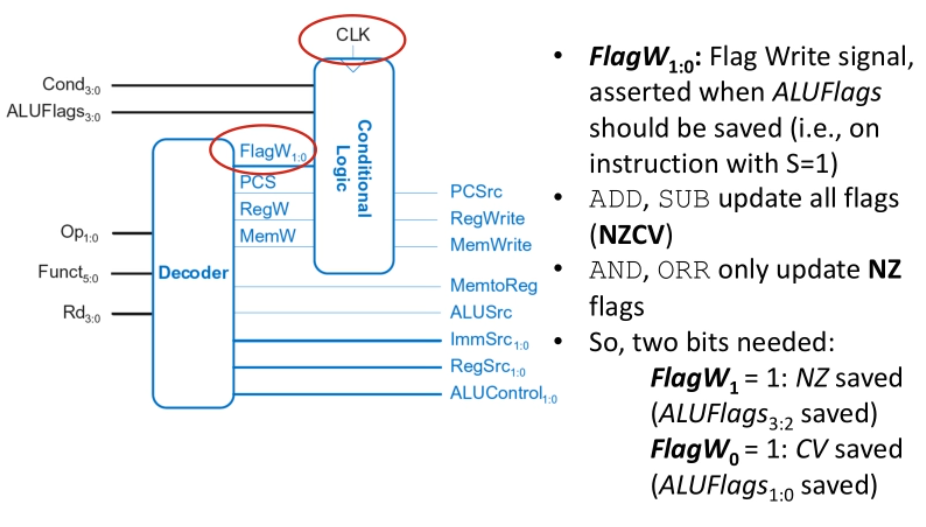
\includegraphics[width=7cm]{ep14.PNG}
                    \end{minipage}
                \item[]
                    \begin{minipage}{0.4\textwidth}
                        Beispiel: \textit{add r1,r2,r3} (1110 $\rightarrow$ always) \\
                        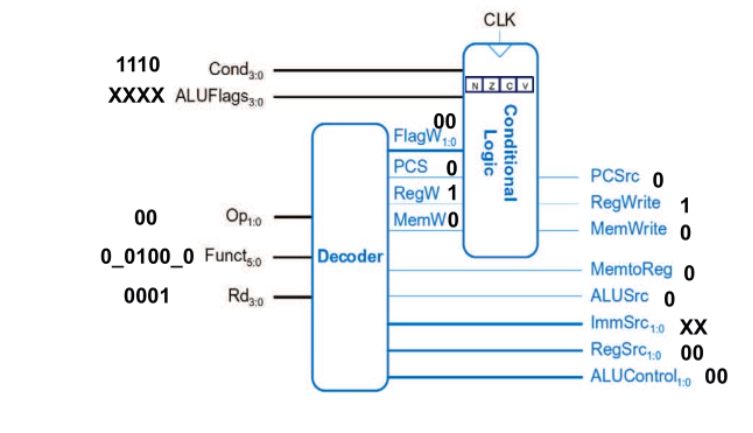
\includegraphics[width=7cm]{ep15.PNG}
                    \end{minipage}
                    \begin{minipage}{0.45\textwidth}
                        Beispiel: \textit{andeq r5,r6,47} \\
                        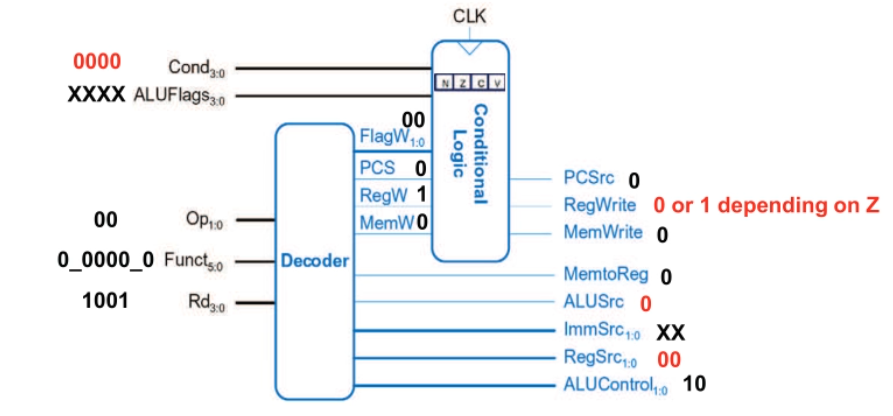
\includegraphics[width=7cm]{ep16.PNG}
                    \end{minipage}
            \end{itemize}

        \item \textbf{Condition Field}
            \begin{itemize}
                \item Verwendung dieser Codes für jeden Befehl als Condition möglich
                \item[] 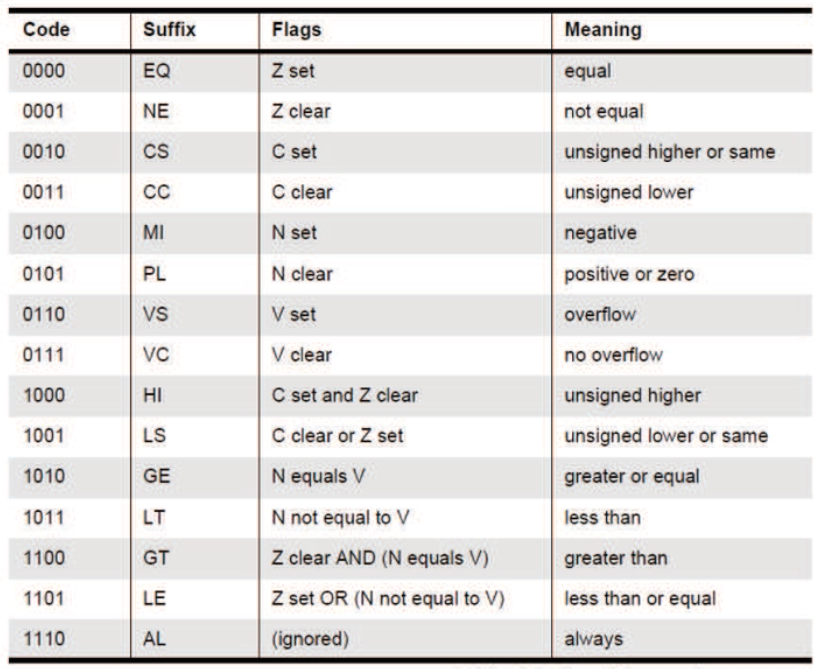
\includegraphics[width=7cm]{conditionfield.PNG}
            \end{itemize}
    \end{itemize}

\subsection{Mehrtakt-Prozessor}
    \begin{itemize}
        \item \textbf{Zustandselemente im Mehrtakt-Prozessor}
            \begin{itemize}
                \item Ersetze getrennte Instruktions- und Datenspeicher (Harvard-Architektur)
                \item durch einen gemeinsamen Speicher (Von-Neumann-Architektur)
                \item[] \includegraphics[width=8cm]{mp1.PNG}
            \end{itemize}

        \item \textbf{Ablauf der Befehlsausführung anhand eines Mehrtaktprozessors}
            \begin{itemize}
                \item Register werden hier zum Zwischenspeichern von Werten genutzt
                \item[] $\Rightarrow$ Damit Wert aufgrund von Takt nicht verloren geht
                \item[]
                    \begin{minipage}{0.4\textwidth}
                        \textit{1. Hole Instruktion (Bsp. ldr)} \\
                        \includegraphics[width=7cm]{mp2.PNG}
                    \end{minipage}
                    \begin{minipage}{0.5\textwidth}
                        \textit{2. Lese Quelle aus Register/Auswertung Direktwert} \\
                        \includegraphics[width=7cm]{mp3.PNG}
                    \end{minipage}
                \item[]
                    \begin{minipage}{0.4\textwidth}
                        \textit{3. Berechne Speicheradresse (Basis + Offset)} \\
                        \includegraphics[width=7cm]{mp4.PNG}
                    \end{minipage}
                    \begin{minipage}{0.5\textwidth}
                        \textit{4. Lese Daten aus Speicher} \\
                        \includegraphics[width=7cm]{mp5.PNG}
                    \end{minipage}
                \item[]
                    \begin{minipage}{0.4\textwidth}
                        \textit{5. Schreibe Daten in Register} \\
                        \includegraphics[width=7cm]{mp6.PNG}
                    \end{minipage}
                    \begin{minipage}{0.5\textwidth}
                        \textit{6. Berechne Adresse nächster Befehl} \\
                        \includegraphics[width=7cm]{mp7.PNG}
                    \end{minipage}
                \item[]
                    \begin{minipage}{0.4\textwidth}
                        \textit{7. Behandlung von r15} \\
                        \includegraphics[width=7cm]{mp8.PNG}
                    \end{minipage}
                    \begin{minipage}{0.5\textwidth}
                        \textit{Erweiterung für str} \\
                        \includegraphics[width=7cm]{mp9.PNG}
                    \end{minipage}
                \item[]
                    \begin{minipage}{0.4\textwidth}
                        \textit{Arithmetische/logische Befehle} \\
                        \includegraphics[width=7cm]{mp10.PNG}
                    \end{minipage}
                    \begin{minipage}{0.5\textwidth}
                        \textit{Sprungbefehl b} \\
                        \includegraphics[width=7cm]{mp11.PNG}
                    \end{minipage}
            \end{itemize}
\pagebreak
        \item \textbf{Datenpfad und Kontrolleinheit}
            \begin{itemize}
                \item[]
                    \begin{minipage}{0.6\textwidth}
                        \includegraphics[width=10cm]{mp12.PNG}
                    \end{minipage}
                    \begin{minipage}{0.3\textwidth}
                        \includegraphics[width=5cm]{mp13.PNG}
                    \end{minipage}
                \item[]
                    \begin{minipage}{0.45\textwidth}
                        \textit{Kontrolleinheit - Detail} \\
                        \includegraphics[width=7cm]{mp14.PNG}
                    \end{minipage}
            \end{itemize}

        \item \textbf{Entwicklung des Steuerwerks}
            \begin{itemize}
                \item Setzen gewisser Steuersignale beim Holen eines Befehls ist notwendig
                \item Steuersignale sind solange 1, wie sie in Zuständen dediziert auf 1 gesetzt sind
                \item[]
                    \begin{minipage}{0.5\textwidth}
                        \includegraphics[width=8cm]{mp15.png}
                    \end{minipage}
                    \begin{minipage}{0.3\textwidth}
                        \includegraphics[width=5cm]{mp16.PNG}
                    \end{minipage}
                \item[]
                    \begin{minipage}{0.45\textwidth}
                        \textit{1. Fetch} \\
                        \includegraphics[width=8cm]{mp17.png}
                    \end{minipage}
                    \begin{minipage}{0.45\textwidth}
                        \textit{2. Decode ldr} \\
                        \includegraphics[width=8cm]{mp18.png}
                    \end{minipage}
                \item[]
                    \begin{minipage}{0.45\textwidth}
                        \textit{3. Execute} \\
                        \includegraphics[width=8cm]{mp20.png}
                    \end{minipage}
                \item[]
                    \begin{minipage}{0.4\textwidth}
                        \includegraphics[width=6cm]{mp19.png}
                    \end{minipage}
                    \begin{minipage}{0.5\textwidth}
                        \includegraphics[width=8cm]{mp21.png}
                    \end{minipage}
                \item \textit{Fetch} und \textit{Decode} sind für alle Befehle gleich
                \item \textit{S4:MemWB} schreibt das Ergebnis, danach wird zum nächsten Befehl übergegangen
                \item 5 versch. Phasen (könnten z.B. 5 Takte sein $\rightarrow$ Überlagern mit Pipelining)
            \end{itemize}

        \item \textbf{Eintakt- vs Mehrtaktprozessor}
            \begin{itemize}
                \item \textit{Gemeinsamkeiten}
                    \begin{itemize}
                        \item \textbf{Datenpfad}: verbindet funktionale Blöcke
                        \item \textbf{Kontrollpfad}: Steuersignale/Steuerwerk
                    \end{itemize}
                \item \textit{Eintakt-Prozessor}
                    \begin{itemize}
                        \item[+] einfach
                        \item[-] Taktfrequenz wird durch langsamste Instruktion bestimmt
                        \item[-] Drei ALUs und zwei Speicher  
                    \end{itemize}
                \item \textit{Mehrtakt-Prozessor}
                    \begin{itemize}
                        \item[+] höhere Taktfrequenz
                        \item[+] einfache Instruktionen laufen schneller
                        \item[+] bessere Wiederverwendung von Hardware in versch. Takten
                        \item[-] aufwendigere Ablaufsteuerung   
                    \end{itemize}
            \end{itemize}
    \end{itemize}

\pagebreak

\subsection{Pipeline-Prozessor}
    \begin{itemize}
        \item \textbf{Befehlsausführung}
            \begin{itemize}
                \item \textit{5 Phasen bei ARM}
                    \begin{itemize}
                        \item Instruction Fetch
                        \item Instruction Decode, Read Register
                        \item Execute ALU
                        \item Memory Read/Write
                        \item Write Register
                    \end{itemize}
                \item Idee: Pipelining dieser Befehlsausführung (siehe unten)
                \item[] \includegraphics[width=10cm]{pipelineIdee.PNG}
            \end{itemize}

        \item \textbf{Abstrakte Darstellung}
            \begin{itemize}
                \item Vereinfachte Darstellung des Datenpfads der Mikroarchitektur
                \item[] \includegraphics[width=12cm]{pipelineAbstrakt.PNG}
                \item \textit{IM}: Instruction Memory
                \item \textit{RF}: Register Field
                \item \textit{DM}: Data Memory
                \item Hinterer Teil grau: lesen / vorderer Teil grau: schreiben 
            \end{itemize}

\pagebreak

        \item \textbf{Datenpfad}
            \begin{itemize}
                \item Einführung von Registern $\rightarrow$ Führt zur Überlappung der Befehlsphasen
                \item[] \includegraphics[width=12cm]{pipelineDaten.PNG}
                \item Führung der Zieladresse über Register (da diese sonst verloren geht)
                \item[] \includegraphics[width=12cm]{pipelineZiel.PNG}
                \item Optimierung der Program Counter Logik
                \item[] \includegraphics[width=12cm]{pipelineProgram.png}
                \item Kontrolleinheit (blau: Kontrollpfad)
                \item[] \includegraphics[width=12cm]{pipelineControl.png}  
            \end{itemize}
    \end{itemize}

\pagebreak

\subsection{Ausnahmebehandlung - Hazards}
    \begin{itemize}
        \item \textbf{Information}
            \begin{itemize}
                \item Treten auf wenn Instruktion auf Ergebnis vorhergehender wartet, dieses aber noch nicht vorhanden ist
                \item \textit{Data Hazard:} z.B. neuer Wert von Register noch nicht in Registerfeld eingetragen
                \item \textit{Control Hazard:} Unklar, welche Instruktion als nächstes ausgeführt wird (Sprünge) 
            \end{itemize}
        
        \item \textbf{Data Hazard}
            \begin{itemize}
                \item Hier: \textit{Read-After-Write Hazard (Raw)} (r1 muss vor Lesen geschrieben werden)
                \item[] \includegraphics[width=10cm]{datahazard.PNG}
                \item \textit{Möglichkeiten:}
                    \begin{itemize}
                        \item Plane Wartezeiten von Anfang an ein (Einfügen von \textit{nops} (no operations) zur Compilezeit)
                        \item Stelle Maschinencode zur Compile-Zeit um (\textit{scheduling/reordering})
                        \item Leite Daten zur Laufzeit schneller über Abkürzungen weiter (\textit{bypassing/forwarding})
                        \item Halte Prozessor zur Laufzeit an bis Daten da sind (\textit{stalling})
                    \end{itemize}
                \item \textit{Einfügen von nops}
                    \begin{itemize}
                        \item[] \includegraphics[width=10cm]{hazardNops.png}
                    \end{itemize}
                \item \textit{Bypassing/Forwarding}
                    \begin{itemize}
                        \item Früheres Einfügen in anderen Pipelinevorgang
                        \item Benötigt Erweitern der Datenpfade
                        \item[]
                            \begin{minipage}{0.45\textwidth}
                                \includegraphics[width=8cm]{hazardBy.PNG}
                            \end{minipage}
                            \begin{minipage}{0.45\textwidth}
                                \includegraphics[width=8cm]{hazardData.png}
                            \end{minipage}
                    \end{itemize}
                \item \textit{Stall}
                    \begin{itemize}
                        \item Wird z.B. bei \texttt{ldr} benötigt
                        \item[] \includegraphics[width=10cm]{dataLdr.PNG}
                        \item Lösung: Pipeline-Stall
                        \item Nachteil: Mehr Cycles / Benötigt auch Anpassung der Datenpfade
                        \item[]
                            \begin{minipage}{0.45\textwidth}
                                \includegraphics[width=8cm]{dataStall.PNG}
                            \end{minipage}
                            \begin{minipage}{0.45\textwidth}
                                \includegraphics[width=8cm]{dataStallData.png}
                            \end{minipage}
                    \end{itemize}
            \end{itemize}
        
        \item \textbf{Control Hazards}
            \begin{itemize}
                \item \string"Leerung\string" der Instruktionen bei Sprungbefehl
                \item[]
                    \begin{minipage}{0.45\textwidth}
                        \textit{Leerung der anderen Instruktionen bei Sprung} \\
                        \includegraphics[width=7cm]{hazardControl1.PNG}
                    \end{minipage}
                    \begin{minipage}{0.45\textwidth}
                        \textit{Optimierung (frühere Feststellung des Sprungs)} \\
                        \includegraphics[width=7cm]{hazardControl2.PNG}
                    \end{minipage}
                \item Anpassung der Datenpfade
                \item[] \includegraphics[width=10cm]{hazardControl3.PNG}
            \end{itemize}
    \end{itemize}

\pagebreak

\section{Gleitkommazahlen/Gleitkommarechenwerte}

\subsection{Gleitkommazahlen}
    \begin{itemize}
        \item \textbf{Zahlendarstellung in Rechnersystemen}
            \begin{itemize}
                \item Unterscheidung zwischen ganzen Zahlen und reellen Zahlen
                \item[] \includegraphics[width=8cm]{zahlendarstellung.png}
            \end{itemize}

        \item \textbf{Darstellung reeller Zahlen}
            \begin{itemize}
                \item \textit{Festkommadarstellung}
                    \begin{itemize}
                        \item Weglassen des Kommas bei der internen Zahlenbildung
                        \item Definierung zu Programmbeginn, bleibt daraufhin fest
                    \end{itemize}
                \item \textit{Gleitkommadarstellung}
                    \begin{itemize}
                        \item Kommastelle ist Bestandteil der Zahl und kann sich verändern
                        \item Standardisiert nach ANSI/IEEE 754 (Keine Angabe des Kommas notwendig)
                        \item Weltweit durchgesetzt - Grundlage für weltweiten Datenaustausch/Rechenwerke
                    \end{itemize}
                \item \textit{Formate Gleitkommadarstellung}
                    \begin{itemize}
                        \item Hinten: Mantisse | s: Vorzeichenbit
                        \item[] \includegraphics[width=10cm]{gleitkommaFormate.PNG}
                        \item Besonderheiten: Null kann durch Normalisierung nicht dargestellt werden
                        \item[] \includegraphics[width=8cm]{gleitkomma0.PNG} 
                    \end{itemize}
            \end{itemize}
    \end{itemize}

\pagebreak

\subsection{Code-Analyse}
    \begin{itemize}
        \item \textit{Beispiel 1:}
            \begin{itemize}
                \item[]
                    \begin{minipage}{0.5\textwidth}
                        \includegraphics[height=4.5cm]{bsp1Code.PNG}
                    \end{minipage}
                    \begin{minipage}{0.4\textwidth}
                        \includegraphics[height=6.5cm]{bsp1Ass.PNG}
                    \end{minipage}
                \item \textit{s-Register}: Single Register (Precision) (32 Bit Register)
                \item \textit{d-Register}: Double Register (Precision) (64 Bit Register)
                \item Speicherung der Konstanten im Dezimalsystem:
                    \begin{itemize}
                        \item[] p = 5.4 $\rightarrow$ 1085066445 $\rightarrow$ 0100 0000 1010 1100 1100 1100 1100 1101 (Umrechnung)
                    \end{itemize}
                \item Neue Befehle und Register:
                    \begin{itemize}
                        \item[] vldr.32, vadd.f32, s14, s15, d7,..
                    \end{itemize}
            \end{itemize}

        \item \textit{Beispiel 2:}
            \begin{itemize}
                \item[]
                    \begin{minipage}{0.5\textwidth}
                        \includegraphics[height=4.5cm]{bsp2Code.PNG}
                    \end{minipage}
                    \begin{minipage}{0.4\textwidth}
                        \includegraphics[height=6.5cm]{bsp2Ass.PNG}
                    \end{minipage}
                \item Speicherung der Konstanten im Dezimalsystem - je 2 32 Bit pro 64 Bit Zahl:
                    \begin{itemize}
                        \item[] p = 5.4 $\rightarrow$ -1717986918\_1075157401
                        \item[] q = 12.6 $\rightarrow$ 858993459\_1076441907
                    \end{itemize}
                \item Neue Befehle und Register:
                    \begin{itemize}
                        \item[] strd, vldr.64, vadd.f64, d6, d7, ...
                    \end{itemize}
            \end{itemize}

        \item \textit{CPU-Informationen unter Linux}
            \begin{itemize}
                \item \texttt{cat /proc/cpuinfo}
                \item \textit{features:} vfp, neon, vfpv3, vfpv4 für Gleitkommazahlen
                \item[] \includegraphics[width=7cm]{cpuinfo.png}
            \end{itemize}
        
    \end{itemize}

\subsection{Studium der Datenblätter/Handbücher}

    \begin{itemize}
        \item \textbf{Suche}
            \begin{itemize}
                \item Suche im Internet nach Datenblättern
                \item Fund: Datenblätter/Handbücher zum Programmiermodell
                \item Fund: Datenblätter/Handbücher zur Hardware-Architektur
            \end{itemize} 

        \item \textbf{Handbuch zum Programmiermodell}
            \begin{itemize}
                \item[]
                    \begin{minipage}{0.3\textwidth}
                        \textit{Registersatz} \\
                        \includegraphics[height=4cm]{registersatz2.png}
                    \end{minipage}
                    \begin{minipage}{0.6\textwidth}
                        \textit{Befehle} \\
                        \includegraphics[height=4cm]{befehle.png}
                    \end{minipage}
                \item[] \textit{Bemerkungen}
                    \begin{itemize}
                        \item Zwei Möglichkeiten Gleitkommazahlen zu verarbeiten
                        \item \textit{Funktionseinheit NEON}
                        \item \textit{Funktionseinheit VFP}
                        \item Beide Funktionseinheiten verwenden selbe Register
                    \end{itemize}
            \end{itemize}

        \item \textbf{Mögliche Realisierung einer Gleitkommaeinheit}
            \begin{itemize}
                \item Auslagerung in sog. Gleitkomma-Coprozessoren (heutzutage in einem Chip)
                \item Diese besitzen iooft separate Instruktions-Pipelines 
                    \begin{itemize}
                        \item Multiplikations und Additions Pipeline (FMAC)
                        \item Divisions und Quadratwurzel Pipeline (DS)
                    \end{itemize}
                \item Pipelines können auch unabhängig voneinander operieren
                \item[]
                    \begin{minipage}{0.45\textwidth}
                        \textit{FMAC-Pipeline} \\
                        \includegraphics[width=7cm]{fmac.png}
                    \end{minipage}
                    \begin{minipage}{0.45\textwidth}
                        \textit{DS-Pipeline} \\
                        \includegraphics[width=7cm]{ds.png}
                    \end{minipage}
                \item \textit{Analyse der Assembler-Köpfe}
                    \begin{itemize}
                        \item Wahl welcher Übersetzung (NEON: \texttt{gcc -mfpu=neon xyz.c})
                        \item[] \includegraphics[width=6cm]{neon.png}
                    \end{itemize}
            \end{itemize}

    \end{itemize}

\subsection{SIMD}

    \begin{itemize}
        \item \textbf{Informationen}
            \begin{itemize}
                \item \textit{SIMD}: Single Instruction Multiple Data
                \item Integration dedizierter Funktionseinheiten in Prozessor zur Beschleunigung von Berechnungen
                \item Für Ganzzahl und Gleitkommazahlen
                \item Beschleunigt z.B. Signalverarbeitung, Video Encodierung, Bildverarbeitung,..
                \item Bei ARM: \textit{NEON}
            \end{itemize}

        \item \textbf{NEON}
            \begin{itemize}
                \item SIMD-Einheit in den ARM Cortex-A Serie Prozessoren
                \item NEON führt \textit{\string"Packed SIMD\string"} aus
                    \begin{itemize}
                        \item Register werden als Vektoren von Elementen desselben Datentyps betrachtet
                        \item Verschiedene Datentypen sind jedoch möglich
                        \item gleichzeitige Ausführung der Befehle in sog. \string"lanes\string"
                    \end{itemize}
                \item \textit{NEON Register}
                    \begin{itemize}
                        \item \textit{AArch32} hat 32 x 64 Bit NEON Register (D0 - D31)
                        \item Diese können auch als 16 x 128 Bit Register gesehen werden (Q0 - Q15)
                        \item[] \includegraphics[width=6cm]{neonRegister.png}
                    \end{itemize}
                \item \textit{NEON Befehle}
                    \begin{itemize}
                        \item Format: V\{<mod>\}<op>\{<shape>\}\{<cond>\}\{.<dt>\}\{<dest>\}, src1, src2
                        \item Modifier (mod): z.B. Q: der Befehl nutzt Saturations-Arithmetik
                    \end{itemize}
                \item \textit{Saturations-Arithmetik}
                    \begin{itemize}
                        \item Resultate werden auf einen festen Bereich zwischen minimalen und maximalen Wert begrenzt
                        \item Kleiner als Minimum $\rightarrow$ Minimum / Grö\ss er als Maximum $\rightarrow$ Maximum
                    \end{itemize}
                \item \textit{Beispiel I}
                    \begin{itemize}
                        \item[] \includegraphics[width=8cm]{neonBsp1.png}
                        \item[] Beide Ausgangsregister 64 Bit, Zielregister 128 Bit (z.B. Multiplikation)
                    \end{itemize}
\pagebreak
                \item \textit{Beispiel II}
                    \begin{itemize}
                        \item[] \includegraphics[width=8cm]{neonBsp2.png}
                        \item[] Ein Ausgangsregister 128 Bit, das Andere 64 Bit, Zielregister 128 Bit
                    \end{itemize}
                \item \textit{Beispiel III}
                    \begin{itemize}
                        \item[] \includegraphics[width=8cm]{neonBsp3.png}
                        \item[] Beide Ausgangsregister, Zielregister 64 Bit (z.B. Multiplikation)
                    \end{itemize}
                \item \textit{Beispielcode}
                    \begin{itemize}
                        \item \texttt{VMULL.S16 Q2, D8, D9}
                    \end{itemize}
                \item \textit{NEON-Programmierung}
                    \begin{itemize}
                        \item NEON optimized libraries
                        \item Vectorizing compilers (gcc)
                        \item NEON intrinsics
                        \item NEON assembly
                    \end{itemize}
            \end{itemize} 

        \item \textbf{Klassifikation von Flynn}
            \begin{itemize}
                \item Aufteilung in sog. \textit{Instruction Streams} und \textit{Data Streams}
                \item Grobe Klassifikation - Aber stark etablierte Begriffe
                \item Verschiedene Aspekte werden nicht oder nur groß erfasst (Pipelining, Wortbreite, Speicher,..)
                \item \textit{Instruction Stream}
                    \begin{itemize}
                        \item SI - Single Instruction
                        \item MI - Multiple Instruction
                    \end{itemize}
                \item \textit{Data Straem}
                    \begin{itemize}
                        \item SD - Single Data
                        \item MD - Multiple Data
                    \end{itemize}
                \item \textit{Kombinationen}
                    \begin{itemize}
                        \item \textit{SISD} - Von-Neumann-Rechner
                        \item \textit{SIMD} - Feldrechner, Vektorrechner
                        \item \textit{MIMD} - Multiprozessorsysteme
                        \item \textit{MISD} - Keine Anwendung
                    \end{itemize}
                \item \textit{Veranschaulichung}
                    \begin{itemize}
                        \item[] \includegraphics[width=7cm]{flynn.png}
                    \end{itemize}
    
            \end{itemize}
    \end{itemize}

\section{Speicher}
\subsection{Speicher}

    \begin{itemize}
        \item \textbf{Bisheriges Modell}
            \begin{itemize}
                \item Drei Phasen der Befehlsausführung
                \item Prozessor mit Registern
                \item Speicher (var1: .word 5)
                \item Hier besteht der Speicher nur aus einem linearen Feld aus Bytes
                \item Die CPU kann auf jede Speicherzelle in konstanter Zeit zugreifen
                \item[] $\Rightarrow$ Einfaches Modell, welches die Realität nicht abbildet
            \end{itemize}
        
        \item \textbf{Speicherhierarchie}
            \begin{itemize}
                \item Lesen und Schreiben in einen Speicher dauert gewisse Zeit
                \item[] $\Rightarrow$ Relativ lang im Vergleich zur Taktfrequenz
                \item Von-Neumann: Daten, Befehle etc müssen alle nacheinander aus dem Speicher geholt werden
                \item Harvard: Obiges kann auch parallel ausgeführt werden
                \item Einführung von Pipelinestufen möglich
                \item \textit{Speicherhierarchie-Pyramide}:
                \item[] \includegraphics[width=8cm]{speicherpyramide.PNG} 
            \end{itemize}

        \item \textbf{Eigenschaften von Speichern}
            \begin{itemize}
                \item \textit{Kosten und Zugriffszeit}
                    \begin{itemize}
                        \item \textit{Kosten:} Messung in Dollar/Bit oder Dollar/MByte
                        \item \textit{Zugriffszeit:} durchschn. Zeit um Wort aus Speicher zu lesen
                        \item \textit{Zykluszeit:} minimale Zeit zwischen zwei Speicherzugriffen
                        \item Das Busprotokoll ist hierfür auch von Relevanz
                        \item \textit{Bandbreite:} Maximale Datenmenge, die pro Sekunde übertragen werden kann (Byte/sec)
                    \end{itemize}
                \item \textit{Geschwindigkeit und Kapazität}
                \item \textit{Zugriffsverfahren}
                    \begin{itemize}
                        \item Zwei verschiedene Zugriffsverfahren
                        \item \textit{Random Access Zugriff}
                            \begin{itemize}
                                \item Register
                                \item Cache-Speicher
                                \item Hauptspeicher
                            \end{itemize}
                        \item \textit{Serieller Zugriff}
                            \begin{itemize}
                                \item Festplatte
                                \item Optische Daten
                                \item Magnetband
                            \end{itemize}
                    \end{itemize}
                \item \textit{Änderbarkeit}
                    \begin{itemize}
                        \item \textit{Read-Only:} Nur Lesen möglich, kein Überschrieben (ROM)
                        \item \textit{Read-Write:} Inhalt kann während des Betriebs geändert werden (RAM)
                        \item \textit{Read-Mostly:} (PROM-Halbleiterspeicher, z.B. für BIOS)
                    \end{itemize}
                \item \textit{Permanenz}
                    \begin{itemize}
                        \item \textit{Flüchtige Speicher:} Inhalt geht bei Stromausfall verloren (Register, Hauptspeicher)
                            \begin{itemize}
                                \item dynamische Speicher: Periodische Erneuerung der Spannung gegen Informationsverlust
                                \item statischer Speicher: Kein Refreshing wie beim dynamischen notwendig
                            \end{itemize}
                        \item \textit{Nicht flüchtige Speicher:} Inhalt bleibt erhalten (ROM, PROM, Festplatte)
                    \end{itemize}
            \end{itemize}
        
        \item \textbf{Speichertechnologien - Random-Access-Memory}
            \begin{itemize}
                \item \textit{Statisches RAM} (SRAM)
                \item \textit{Dynamisches RAM} (DRAM)
                \item SRAM schneller und deutlich teurer als DRAM
                \item SRAM $\Rightarrow$ Cache / DRAM $\Rightarrow$ Hauptspeicher
                \item Verteilung meist: 12MB SRAM / 8GB+ DRAM
                \item[]
                    \begin{minipage}{0.4\textwidth}
                        \item \textit{Organisation des Speichers}
                        \item[] \includegraphics[width=7cm]{speicherOrga.PNG}
                    \end{minipage}
                    \begin{minipage}{0.5\textwidth}
                        \begin{itemize}
                            \item Cellarray mit Rows und Columns
                            \item Wordline: 32 Bit Wort z.B.
                            \item Storage Cell: speichert 1 Bit (0/1)
                            \item Auswahl über Zeilenadresse + Bitline
                            \item Amplifier: Verstärkung geringer Spannungen
                            \item Ausgabe: Diskrete 0 oder 1
                        \end{itemize}
                    \end{minipage}
            \end{itemize}

        \item \textbf{Statisches RAM}
            \begin{itemize}
                \item Speichert Informationen solange, wie Spannungsversorgung angeschaltet ist
                \item Bistabile Schaltung (zwei stabile Zustände) (wird nicht so in der Klausur abgefragt)
                \item 6T Zelle wegen 6 Transistoren
                \item[] \includegraphics[width=5cm]{staticRam1.png}
            \end{itemize}

\pagebreak

        \item \textbf{Dynamisches RAM}
            \begin{itemize}
                \item Speichert Informationen in einem Kondensator
                \item Bezeichnung als 1T-Zelle
                \item Refresh-Zyklus notwendig, da Kondensator sich entleert
                \item[]
                    \begin{minipage}{0.45\textwidth}
                        \includegraphics[width=7cm]{dynamicRam1.PNG}
                    \end{minipage}
                    \begin{minipage}{0.45\textwidth}
                        \includegraphics[width=7cm]{dynamicRam2.PNG}
                    \end{minipage}
            \end{itemize}
    \end{itemize}

\subsection{Speicherorganisation}
    \begin{itemize}
        \item \textbf{Bezeichnungen}
            \begin{itemize}
                \item Eigenschaften eines RAM-Chips werden durch zwei Grö\ss en gegeben
                    \begin{itemize}
                        \item \textit{Anzahl adressierbarer Plätze}
                        \item \textit{Breite in Bit jedes adressierbaren Platzes}
                    \end{itemize}
                \item \textit{Bsp: 256K x 1 SRAM}
                    \begin{itemize}
                        \item 256K Einträge mit 1 Bit Breite
                        \item 256K = $2^18$ $\rightarrow$ 18 Adresseingänge + 1 Bit Dateneingang/ausgang
                    \end{itemize}
                \item \textit{Bsp: 32K x 8 SRAM}
                    \begin{itemize}
                        \item 32K Einträge mit 8 Bit Breite
                        \item 32K = $2^15$ $\rightarrow$ 15 Adresseingänge + 8 Bit Dateneingang/ausgang
                        \item[] \includegraphics[width=7cm]{32kx8.png}
                    \end{itemize}
            \end{itemize}

\pagebreak

        \item \textbf{Abstrakte Darstellung eines 128 Bit 16x8 DRAM Chips}
            \begin{itemize}
                \item[] \includegraphics[width=8cm]{dram.png}
                \item[] 16 Felder, 8 Bit Dateneingang/ausgang 
                \item[]
                    \begin{minipage}{0.45\textwidth}
                        \textit{Auswahl der Reihe - RAS (Row Adress Strobe)} \\
                        \includegraphics[width=7cm]{ras.png}
                    \end{minipage}
                    \begin{minipage}{0.45\textwidth}
                        \textit{Auswahl der Spalte - CAS (Column Adress Strobe)}
                        \includegraphics[width=7cm]{cas.png}
                    \end{minipage}
            \end{itemize}

        \item \textbf{Verschaltung mehrerer Speichermodule}
            \begin{itemize}
                \item[] \includegraphics[width=10cm]{speichermodule.png}
            \end{itemize}

        \item \textbf{Verbindung von CPU und Speicher}
            \begin{itemize}
                \item[] \includegraphics[width=10cm]{verbindung.png}
            \end{itemize}
    \end{itemize}
\subsection{Lokalität}

    \begin{itemize}
        \item \textbf{Informationen}
            \begin{itemize}
                \item Lokalität ist wichtig für eine funktionierende Speicherhierarchie
                \item \textit{Lokalitätsprinzip:}
                \item[] Bei Programmausführung wird nur auf einen geringen Teil des Adressraumes zugegriffen
                \item[] \includegraphics[width=8cm]{lokalität1.png} 
            \end{itemize}

        \item \textbf{Formen der Lokalität}
            \begin{itemize}
                \item \textit{zeitliche (temporale) Lokalität}
                    \begin{itemize}
                        \item Nach Zugriff auf Daten wird mit großer Wahrscheinlichkeit bald wieder darauf zugegriffen
                        \item Bsp.: Schleifen
                    \end{itemize}
                \item \textit{räumliche Lokalität}
                    \begin{itemize}
                        \item Sukzessiver Zugriff auf Daten, die in der Nähe liegen
                        \item Bsp.: sequentielle Instruktionsfolgen (ohne Sprünge)
                        \item Bsp.: Reihungen, Matrizen
                    \end{itemize}
            \end{itemize}

        \item \textbf{Vorteile}
            \begin{itemize}
                \item Gut geschriebene Programme haben eine gute Lokalität
                \item Hat hohe Auswirkung auf die Performanz (bessere Lokalität $\rightarrow$ schneller)
                \item Lokalität der Daten / Lokalität der Befehle
            \end{itemize}

        \item \textbf{Beispiel 1 - Summe eines Vektors}
            \begin{itemize}
                \item[]
                    \begin{minipage}{0.35\textwidth}
                        \begin{minted}[autogobble]{c}
                        int sumvec (int v[N])
                        {
                            ...
                            int i, sum = 0;

                            for (i = 0; i < N; i++)
                                sum += v[i];
                            return sum;
                            ...
                        }
                        \end{minted}
                    \end{minipage}
                    \begin{minipage}{0.5\textwidth}
                        \includegraphics[width=7cm]{lokalitätbsp1.png}
                        \begin{itemize}
                            \item Gute räumliche Lokalität
                            \item Schlechte zeitliche Lokalität (1x Zugriff)
                            \item (i allerdings gute zeitliche Lokalität)
                        \end{itemize}
                    \end{minipage}
            \end{itemize}

        \item \textbf{Beispiel 2 - Summe eines Arrays}
            \begin{itemize}
                \item[]
                    \begin{minipage}{0.35\textwidth}
                        \begin{minted}[autogobble]{c}
                        int sumvec (int v[N])
                        {
                            ...
                            int sumarrayrows(int a[M][N])
                            {
                                int i,j,sum = 0;
                                for (i = 0; i < M; i++)
                                    for (j = 0; j < N; j++)
                                        sum += a[i][j];
                                return sum;
                            }
                            ...
                        }
                        \end{minted}
                    \end{minipage}
                    \begin{minipage}{0.5\textwidth}
                        \includegraphics[width=7cm]{lokalitätbsp2.png}
                        \begin{itemize}
                            \item Gute räumliche Lokalität
                            \item Schlechte zeitliche Lokalität (1x Zugriff)
                            \item (i allerdings gute zeitliche Lokalität)
                        \end{itemize}
                    \end{minipage}
            \end{itemize}

\pagebreak

        \item \textbf{Beispiel 3 - Summe eines Arrays}
            \begin{itemize}
                \item[]
                    \begin{minipage}{0.35\textwidth}
                        \begin{minted}[autogobble]{c}
                        int sumvec (int v[N])
                        {
                            ...
                            int sumarrayrows(int a[M][N])
                            {
                                int i,j,sum = 0;
                                for (i = 0; i < N; i++)
                                    for (j = 0; j < M; j++)
                                        sum += a[i][j];
                                return sum;
                            }
                            ...
                        }
                        \end{minted}
                    \end{minipage}
                    \begin{minipage}{0.5\textwidth}
                        \includegraphics[width=7cm]{lokalitätbsp3.png}
                        \begin{itemize}
                            \item Schlechte räumliche Lokalität (Springen im Speicher)
                            \item Schlechte zeitliche Lokalität (1x Zugriff)
                            \item (i allerdings gute zeitliche Lokalität)
                        \end{itemize}
                    \end{minipage}
            \end{itemize}

        \item \textbf{Lokalität der Befehle}
            \begin{itemize}
                \item Befehle sind auch im Speicher abgelegt, hier auch gute Lokalität möglich
                \item Für die for Schleifen der Beispiele gilt gute räumliche Lokalität
                \item Schleifenkörper wiederholt ausgeführt $\rightarrow$ gute zeitliche Lokalität
            \end{itemize}

        \item \textbf{Beispiel 4/5 - Zeilenweises/Spaltenweises Schreiben in ein Array}
            \begin{itemize}
                \item[]
                    \begin{minipage}{0.45\textwidth}
                        \textit{Zeilenweises Schreiben eines Arrays}
                        \begin{minted}[autogobble]{c}
                        int main()
                        {
                            register long i,j;
                            static long matrix[DIM][DIM];

                            for (i = 0; i < DIM; i++)
                                for (j = 0; j < DIM; j++)
                                    matrix[i][j] = 0;

                            return 0;
                        }
                        \end{minted}
                    \end{minipage}
                    \begin{minipage}{0.45\textwidth}
                        \textit{Spaltenweises Schreiben eines Arrays}
                        \begin{minted}[autogobble]{c}
                        int main()
                        {
                            register long i,j;
                            static long matrix[DIM][DIM];

                            for (j = 0; j < DIM; j++)
                                for (i = 0; i < DIM; i++)
                                    matrix[i][j] = 0;

                            return 0;
                        }
                        \end{minted}
                    \end{minipage}
                \item[] $\Rightarrow$ Zeilenweises Schreiben um Einiges schneller als spaltenweises
            \end{itemize}

        
    \end{itemize}

\pagebreak

\subsection{Prinzip des Caches}

    \begin{itemize}
        \item \textbf{Informationen}
            \begin{itemize}
                \item Kleiner, schneller Speicher (SRAM)
                \item Prozess einen Cache zu benutzen: \textit{caching}
                \item Schneller, kleinerer Speicher auf Level $k$ fungiert als Cache für langsameren, schnelleren Speicher auf Level $k+1$
                \item Wird mehrfach angewendet (siehe Speicherhierarchie)
            \end{itemize}

        \item \textbf{Prinzip des Cachings}
            \begin{itemize}
                \item[] \includegraphics[width=10cm]{caching.png}
                \item Laden ganzer Wordlines $\rightarrow$ Lokalität sehr wichtig
            \end{itemize}

        \item \textbf{Cache Hits}
            \begin{itemize}
                \item Programm benötigt Daten vom Objekt $d$
                \item[] $\Rightarrow$ Überprüfen, ob $d$ in einem der Blöcke auf Level $k$ gespeichert ist
                \item Wenn $d$ gefunden wird $\Rightarrow$ \textbf{Cache Hit}
                \item $k$ schneller als $k+1$ $\Rightarrow$ Geschwindigkeitsvorteil
                \item (Auch Geschwindigkeitsunterschiede zwischen L1, L2, L3 (Speicherpyramide))
            \end{itemize}

        \item \textbf{Cache Misses}
            \begin{itemize}
                \item Programm benötigt Daten vom Objekt $d$
                \item[] $\Rightarrow$ Überprüfen, ob $d$ in einem der Blöcke auf Level $k$ gespeichert ist
                \item Wenn $d$ nicht gefunden wird $\Rightarrow$ \textbf{Cache Miss}
                \item Cache auf Level $k$ holt dann Block mit $d$ von Cache auf Level $k+1$
                \item Falls Cache auf Level $k$ bereits voll $\Rightarrow$ Überschreiben (Ersetzung)
                \item Unterschiedliche Strategien für Blockersetzung (Zufall, Least-Recently-Used (LRU))
            \end{itemize}

        \item \textbf{Blick auf Speicherhierarchie}
            \begin{itemize}
                \item[] Blöcke und Latenz werden nach unten hin größer
                \item[] \includegraphics[width=8cm]{cachingSpeicher.png} 
            \end{itemize}
    \end{itemize}

\subsection{Cachehierarchie ARM / Intel Core i7 }

    \begin{itemize}
        \item[]
            \begin{minipage}{0.4\textwidth}
                \textit{Speicheraufbau} \\
                \includegraphics[width=7cm]{speicheraufbau.png}
            \end{minipage}
            \begin{minipage}{0.45\textwidth}
                \begin{itemize}
                    \item Jeder Kern hat eigenen Registersatz
                    \item d-Cache: Datencache
                    \item i-Cache: Instruktionscache
                \end{itemize}
            \end{minipage}
    \end{itemize}
\end{document}